% !TEX program = xelatex
\IfFileExists{main.tex}{\documentclass[main.tex]{subfiles}}{
  \IfFileExists{../../main.tex}{\documentclass[../../main.tex]{subfiles}}{
    \IfFileExists{../main.tex}{\documentclass[../main.tex]{subfiles}}{
      \documentclass[Book\space NL/main.tex]{subfiles}
    }
  }
}

\begin{document}
\ifSubfilesClassLoaded{
  \ifcsname appendixchapterparent\endcsname
  \else
    \standaloneappendixchaptersetup{C}{2}
  \fi
}{}
\chapter{Virology: Viruses and Viral Diseases}
\labch{appendix-c2-virology}
\index{virus!general principles}
{}\margintoc{}

While the preceding sections of our text discuss medical microbiology from a systems-based perspective, this section introduces the foundations of medical virology and provides an overview of this ever-expanding field. This section is designed to present a ``microbe parade'' of sorts (following Murray's approach\footnote{Hopefully it is abundantly clear that we intend to focus on knowledge with greatest relevance in practice for the Southeast Asian practitioner.}) and act as a summary of the knowledge presented in the preceding sections.

Personally, I find that medical microbiology is one of the most difficult topics in all of clinical medicine, if not the most difficult, thanks in part to the massive body of knowledge that must be remembered and understood by medical students. As such, I hope that this section serves as a starting point for students looking to develop their understanding and more effectively tackle examinations involving virology and the pathophysiology of infection. Additionally, I note with thanks that the medical virology section of this text is based on the core concepts presented in Section 5 (``Virology,'' chapters 35--56) of \textit{Medical Microbiology}, 10th ed., by \textcite{Murray2026MedicalMicrobiology}.

Content coverage of this topic is as follows [quoted verbatim, sic. from specifications]:
\begin{itemize}
  \item B1.5.1 --- Principles of medical microbiology and parasitology
  \begin{enumerate}
    \item Human pathogen classification (bacteria, virus, fungus, parasite, prion)
    \item Basic Human microbiota
    \item Basic biosafety for general practitioner (Biosafety Level, Personal protective equipment, sterilization, disinfection)
    \item Microbes in medical biotechnology applications (probiotics, viral vector vaccine, gene therapy, oncolytic virus, phage therapy)
    \item Vectors control, and prevention (mosquito, flea, tick, mite and fly)
    \item Emerging infectious diseases (e.g., COVID 19)
    \item Principle of drug resistance pathogens
    \item Principle of serologic studies
    \item Principles of molecular diagnosis
  \end{enumerate}
  \item B1.5.3 --- General Principles of medical virology
  \begin{enumerate}
    \item Classification of Medically Important Viruses
    \item Structure, genome (general concept for understanding antivrial agents, vaccine)
    \item Replication (general concept for understanding antiviral agents, antibody)
    \item Pathogenisis
    \item Principles of cultivation, assay and laboratory diagnosis
    \item Zoonosis, vector-bourne disease of pathogenic virus: dengue hemorrhagic fever, zika, Japanese encephalitis, chikungunya, rabies
  \end{enumerate}
\end{itemize}

\reftab{virology_nl_content_alignment} compares these content objectives with what this chapter currently covers.

\begin{center}
\captionof{table}{Alignment of the virology chapter with NL content objectives. Source: Medical Council Notification 12/2555, Part 1A; coverage reflects the current content of this chapter.}
\labtab{virology_nl_content_alignment}
\footnotesize
\setlength{\tabcolsep}{2pt}
\renewcommand{\arraystretch}{1.12}
\begin{tabular}{@{}>{\RaggedRight\arraybackslash}p{0.14\textwidth}>{\RaggedRight\arraybackslash}p{0.44\textwidth}>{\RaggedRight\arraybackslash}p{0.39\textwidth}@{}}
\toprule
\textbf{NL code} & \textbf{Content objective} & \textbf{Coverage in this chapter} \\
\midrule
B1.5.7.1 & Microbial classification & Partial: viral genome grouping is introduced; broader microbial classification and formal virus taxonomy need further coverage. \\
B1.5.7.3 & Viruses and viral diseases & Partial: foundational virology and classification are introduced; detailed replication and clinical disease content remain to be covered. \\
B1.5.7.3.1 & Physical and chemical properties & Partial: capsid and envelope structure and environmental stability are introduced, but properties are not reviewed systematically. \\
B1.5.7.3.2 & Replication & Partial: host-cell dependence and Baltimore routes to mRNA are introduced; complete replication cycles remain to be covered. \\
B1.5.7.3.3 & Genetics & Partial: DNA/RNA genome types are introduced; viral genetics and genetic variation are not covered. \\
B1.5.7.3.4 & Principles of cultivation, assay, and laboratory diagnosis & Not yet covered. \\
B1.5.7.3.5 & Molecular basis of pathogenesis & Partial: immune evasion is mentioned, but mechanisms of pathogenesis are not explained. \\
B1.5.7.3.6 & Pathophysiology of infection & Not yet covered. \\
B1.5.7.3.7 & Latent and persistent infections & Not yet covered. \\
B1.5.7.3.8 & Epidemiology & Partial: general transmission routes are listed; virus-specific epidemiology is not covered. \\
B1.5.7.3.9 & Oncogenic viruses & Not yet covered. \\
B1.5.7.3.10 & Viral diseases not classified in the system: dengue haemorrhagic fever and chikungunya fever; varicella; zoster; herpes simplex infection; viral exanthems (measles, rubella, erythema infectiosum, exanthema subitum, and hand, foot, and mouth disease); mumps; infectious mononucleosis; and cytomegaloviral infection & Not yet covered: these diseases are not discussed clinically. \\
\bottomrule
\end{tabular}
\end{center}



\section{High-yield viral pathogen reference}
\label{sec:viral-pathogen-reference}
\index{virus!reference table}
\index{virus!diagnosis!summary reference}
\index{virus!pathogens}

The following table consolidates the virus notes in the accompanying review workbook; see Table~\ref{tab:viral-pathogen-summary}. Supplementary descriptions are drawn from standard references~\parencite{Murray2026MedicalMicrobiology}. Grey text indicates the Molluscum diagnostic detail that was not listed in the class materials. Mpox treatment notes follow current CDC clinical guidance~\parencite{CDC2026MpoxCare}; dengue diagnosis and care notes follow CDC guidance~\parencite{CDC2025DengueTesting,CDC2026DengueCare}; rabies post-exposure prevention should follow current national guidance~\parencite{CDC2026RabiesPEP}. Refer to Table~\ref{tab:viral-pathogen-summary} and the relevant sections above for fuller discussion.

\pagelayout{wide}
\begingroup
\footnotesize
\setlength{\tabcolsep}{3pt}
\renewcommand{\arraystretch}{1.15}
\begin{longtable}{@{}>{\RaggedRight\arraybackslash}p{0.18\linewidth}>{\RaggedRight\arraybackslash}p{0.21\linewidth}>{\RaggedRight\arraybackslash}p{0.30\linewidth}>{\RaggedRight\arraybackslash}p{0.25\linewidth}@{}}
\caption[Selected viruses: high-yield reference]{Selected viruses: genome, transmission, clinical features, diagnosis, and prevention or treatment.}\label{tab:viral-pathogen-summary}\\
\toprule
\textbf{Virus / genome} & \textbf{Transmission / incubation} & \textbf{Clinical features / diagnostic clues} & \textbf{Treatment / prevention} \\
\midrule
\endfirsthead
\caption[]{Selected viruses: high-yield reference (continued).}\\
\toprule
\textbf{Virus / genome} & \textbf{Transmission / incubation} & \textbf{Clinical features / diagnostic clues} & \textbf{Treatment / prevention} \\
\midrule
\endhead
\midrule
\multicolumn{4}{r}{\footnotesize Continued on next page}\\
\endfoot
\bottomrule
\endlastfoot
\textbf{Variola virus}\index{variola virus}\index{virus families!Orthopoxvirus} (Orthopoxvirus); enveloped linear dsDNA & Respiratory exposure and direct contact with lesions or contaminated materials; typically 10--12 days. No animal reservoir. & Febrile prodrome followed by deep-seated vesicles or pustules, usually at the same stage of development and with centrifugal distribution. Vesicle fluid or scabs: NAAT. Chickenpox is an important differential. & Smallpox has been eradicated. Vaccination is reserved for specific public-health or occupational indications.\\
\textbf{Mpox virus}\index{mpox virus}\index{virus families!Orthopoxvirus} (Orthopoxvirus); enveloped linear dsDNA & Direct contact with lesions, body fluids, or contaminated materials; zoonotic and human-to-human transmission; typically 6--13 days. & Fever, lymphadenopathy, and a rash 1--3 days after fever onset, with firm, deep-seated, well-circumscribed and often umbilicated lesions. Clades I and II differ in their epidemiology and reported severity; outbreak case-fatality varies by setting. Lesion swabs, vesicle fluid, or crusts: NAAT. & Most patients receive supportive care and pain control. Tecovirimat may be considered for patients with severe disease or at high risk under specialist/public-health guidance; brincidofovir is an additional option in selected severe cases. Vaccination is recommended for eligible risk groups according to local guidance.\\
\textbf{Molluscum contagiosum virus}\index{molluscum contagiosum virus}\index{virus families!Molluscipoxvirus} (Molluscipoxvirus); enveloped linear dsDNA & Direct skin-to-skin or sexual contact; incubation approximately 2 weeks to 6 months. & Painless, pearly or flesh-coloured umbilicated papules, particularly in children and immunocompromised people. Biopsy may show Henderson--Patterson (molluscum) bodies in keratinocytes. \textcolor{black!55}{The workbook notes that this diagnostic detail was not included in the class materials.} & Usually self-limiting. Treatment is generally reserved for selected symptomatic, extensive, or persistent lesions.\\
\textbf{Parvovirus B19}\index{parvovirus B19}\index{virus families!Parvoviridae} (Erythrovirus); non-enveloped linear ssDNA & Respiratory droplets, blood products, and vertical transmission; the workbook records an incubation of 6--11 days. & Febrile prodrome; slapped-cheek rash in children; arthralgia; and transient aplastic crisis due to infection of erythroid precursors (pure red cell aplasia). Dog-ear pronormoblasts may be seen. Fetal infection can cause anaemia, hydrops fetalis, and fetal loss. Serology or PCR. & Usually supportive. Assess pregnant patients and people with haemolytic or immunocompromising conditions carefully.\\
\textbf{Hepatitis A virus (HAV)}\index{hepatitis A virus}\index{virus families!Hepatovirus} (Hepatovirus); non-enveloped linear $+$ssRNA & Faecal--oral transmission, including contaminated food and water; incubation typically 3--6 weeks. & Often asymptomatic in children; acute hepatitis and jaundice are more common in adults. Anti-HAV IgM supports acute infection. & Vaccination, hygiene, and immune globulin for selected indications. Treatment is supportive; liver transplantation is rarely required for fulminant failure.\\
\textbf{Hepatitis B virus (HBV)}\index{hepatitis B virus}\index{virus families!Orthohepadnavirus} (Orthohepadnavirus); enveloped, partially double-stranded circular DNA & Blood, blood products, sexual contact, and vertical transmission; incubation typically 2--3 months. & Acute or chronic hepatitis; chronic infection can lead to cirrhosis and hepatocellular carcinoma. Assess HBsAg, anti-HBc, anti-HBs, HBeAg, and HBV DNA as appropriate. Ground-glass hepatocytes may be seen histologically. & Vaccination prevents infection. Acute infection is usually managed supportively; chronic infection may require nucleos(t)ide analogues or interferon-based treatment.\\
\textbf{Hepatitis C virus (HCV)}\index{hepatitis C virus}\index{virus families!Hepacivirus} (Hepacivirus); enveloped linear $+$ssRNA & Mainly blood-borne, including injecting drug use, needlestick injury, tattoos or body piercing, and unscreened transfusion; sexual and vertical transmission are less common. & Frequently persistent infection, with risk of cirrhosis, liver failure, and hepatocellular carcinoma. Lack of proofreading by the viral polymerase promotes mutation; genotype 3 is common in Southeast Asia. Screen with anti-HCV antibody (or antigen where available) and confirm current infection with HCV RNA. & Blood-donor screening and harm-reduction measures. Direct-acting antiviral regimens can cure most infections.\\
\textbf{Hepatitis D virus (HDV)}\index{hepatitis D virus}\index{virus families!Deltavirus} (Deltavirus); circular, negative-sense ssRNA with an HBV-derived envelope & Blood and blood-product exposure; occurs as co-infection with HBV or superinfection in a person with chronic HBV. & Defective virus that requires HBV surface antigen to complete its infectious cycle. Co-infection or superinfection may cause more severe hepatitis. Test anti-HDV and HDV RNA in people with HBV. & HBV vaccination prevents HDV infection. Management of established HDV requires specialist assessment; interferon-alpha therapy may be considered in selected cases.\\
\textbf{Hepatitis E virus (HEV)}\index{hepatitis E virus}\index{virus families!Orthohepevirus} (Orthohepevirus); non-enveloped linear $+$ssRNA & Mainly faecal--oral, often water-borne; zoonotic food-borne transmission occurs through undercooked pork or organ meat. The workbook records an incubation of about 40 days. & Similar to HAV, with acute hepatitis and jaundice; severe disease is a concern in pregnancy, and chronic infection can occur in some immunocompromised people. It is not usually blood-borne. Anti-HEV IgM or HEV RNA in stool or liver tissue. & Usually supportive. Ribavirin may be considered by specialists for selected chronic or severe cases.\\
\textbf{Poliovirus}\index{poliovirus}\index{virus families!Enterovirus} (Enterovirus); non-enveloped linear $+$ssRNA & Faecal--oral, oral--oral, and food- or water-borne transmission; humans are the only natural host. & Ranges from asymptomatic infection to aseptic meningitis and acute flaccid paralysis. Structural proteins: VP1 binds the CD155 receptor; VP2 and VP3 support capsid structure; VP4 stabilises the inner capsid and genome. Replication proteins include 2A (host-protein synthesis shut-off), 2B (membrane effects), VPg/3B (RNA-synthesis primer), 2C (ATPase/helicase), and 3D (RNA-dependent RNA polymerase). Stool is preferred for PCR or virus isolation. & Oral and inactivated polio vaccines are used in immunisation programmes. There is no specific antiviral treatment.\\
\textbf{Rabies virus}\index{rabies virus}\index{virus families!Lyssavirus} (Lyssavirus); enveloped, linear negative-sense ssRNA & Saliva from an infected mammal, usually through a bite or scratch; incubation is commonly weeks to months but may be longer. & Prodrome followed by progressive neurological disease, including hydrophobia or aerophobia, and encephalitis. Ante-mortem testing may include RT-PCR and direct fluorescent antibody testing; Negri bodies are a post-mortem histological finding. & Immediate wound cleansing and prompt post-exposure prophylaxis, including vaccine and rabies immunoglobulin when indicated. Vaccination and animal control prevent exposure.\\
\textbf{Human papillomavirus (HPV)}\index{human papillomavirus}\index{virus families!Papillomaviridae} (Papillomaviridae); non-enveloped circular dsDNA & Mainly sexual or other intimate skin-to-skin contact; vertical transmission can also occur. & Anogenital warts and HPV-associated cancers. E5, E6, and E7 oncoproteins affect cell growth and tumour-suppressor pathways. Cervical cytology (Pap test; Bethesda classification), HPV PCR, and biopsy of suspicious lesions are used as appropriate. & HPV vaccination and cervical screening.\\
\textbf{JC polyomavirus}\index{JC polyomavirus}\index{virus families!Polyomaviridae}; non-enveloped circular dsDNA & Usually acquired early in life; transmission route is not fully established. Reactivation occurs with impaired cellular immunity. & Reactivation may cause progressive multifocal leukoencephalopathy (PML). CSF JC-virus PCR supports diagnosis. & No reliably effective direct antiviral treatment; management focuses on restoring immune function where possible.\\
\textbf{BK polyomavirus}\index{BK polyomavirus}\index{virus families!Polyomaviridae}; non-enveloped circular dsDNA & Usually acquired early in life; reactivation is particularly important after transplantation. & Can cause polyomavirus-associated nephropathy and haemorrhagic cystitis. Urine and plasma PCR are used for assessment and monitoring. & Specialist-guided reduction of immunosuppression where appropriate; monitor renal function and viral load.\\
\textbf{Merkel cell polyomavirus}\index{Merkel cell polyomavirus}\index{virus families!Polyomaviridae}; non-enveloped circular dsDNA & Persistent infection; the precise transmission route is not fully established. & Associated with Merkel cell carcinoma. Diagnosis is based on tumour histopathology and appropriate immunohistochemistry. & Management follows specialist skin-cancer guidance.\\
\textbf{Human T-lymphotropic virus 1 (HTLV-1)}\index{human T-lymphotropic virus 1}\index{virus families!Retroviridae}; enveloped diploid $+$ssRNA retrovirus & Sexual contact, blood exposure, and breastfeeding. & Often asymptomatic; associated with adult T-cell leukaemia/lymphoma and HTLV-1-associated myelopathy/tropical spastic paraparesis. Tax-1 and HBZ contribute to disease mechanisms. Serology with confirmatory testing. & Prevention includes screened blood products, safer sex, and counselling about vertical transmission. Specialist management of associated disease.\\
\textbf{Mumps virus}\index{mumps virus}\index{virus families!Orthorubulavirus} (Orthorubulavirus); enveloped, non-segmented negative-sense ssRNA & Respiratory droplets and close contact; incubation commonly 16--18 days. & Parotitis; complications include orchitis, meningitis, encephalitis, and hearing loss. Buccal-swab RT-PCR is preferred where available. & MMR vaccination, droplet precautions, and supportive care.\\
\textbf{Measles virus}\index{measles virus}\index{virus families!Morbillivirus} (Morbillivirus); enveloped, non-segmented negative-sense ssRNA & Airborne transmission; incubation to rash is usually about 10--14 days. & Cough, coryza, conjunctivitis, Koplik spots, and a generalised rash. RT-PCR and serology support diagnosis. & MMR vaccination, airborne precautions, vitamin A in appropriate clinical settings, and supportive care.\\
\textbf{Rubella virus}\index{rubella virus}\index{virus families!Rubivirus} (Rubivirus, Matonaviridae; formerly classified in Togaviridae); enveloped $+$ssRNA & Respiratory droplets; vertical transmission can cause congenital rubella syndrome. & Mild fever and rash; fetal infection can cause congenital abnormalities. Serology and RT-PCR are used as appropriate. & MMR vaccination and droplet precautions.\\
\textbf{Human parainfluenza viruses (HPIV 1--4)} (Respirovirus / Orthorubulavirus); enveloped negative-sense ssRNA & Respiratory droplets and contact with respiratory secretions. & Common causes of croup and other respiratory tract infections, especially in children. NAAT can identify the virus. & Supportive care and respiratory infection-control precautions.\\
\textbf{Hendra and Nipah viruses}\index{Hendra virus}\index{Nipah virus}\index{virus families!Henipavirus} (Henipavirus); enveloped negative-sense ssRNA & Zoonotic transmission from infected animals or contaminated materials; person-to-person spread can occur, particularly with Nipah virus. & Can cause severe respiratory disease and encephalitis. Diagnosis requires specialist molecular testing and public-health laboratory coordination. & No routinely available specific antiviral treatment; strict infection-control and public-health measures are essential.\\
\textbf{Influenza A(H1N1)}\index{influenza A(H1N1)}\index{virus families!Orthomyxoviridae}; enveloped, segmented negative-sense ssRNA & Respiratory droplets and aerosols; incubation is commonly 1--4 days. & Influenza-like illness, including fever, myalgia, cough, and respiratory symptoms. NAAT is used for confirmation when indicated. The H1N1 subtype includes the 2009 pandemic strain and seasonal descendants. & Annual influenza vaccination and antivirals for selected patients according to current guidance.\\
\textbf{Avian influenza A(H7N9)}\index{avian influenza A(H7N9)}\index{virus families!Orthomyxoviridae}; enveloped, segmented negative-sense ssRNA & Mainly zoonotic exposure to infected birds or contaminated environments. & May cause severe lower-respiratory disease. Diagnosis requires molecular testing and public-health assessment. & Infection prevention, exposure control, and specialist/public-health management.\\
\textbf{Dengue virus}\index{dengue virus}\index{virus families!Flavivirus} (Flavivirus); enveloped $+$ssRNA & Aedes mosquitoes; incubation commonly 4--10 days. & Fever, severe headache, retro-orbital pain, myalgia, arthralgia, and rash; severe disease may involve plasma leakage or bleeding. During days 0--7, use NAAT plus IgM or NS1 antigen plus IgM; after day 7, IgM is the primary test. CBC supports monitoring. & No specific antiviral treatment. Supportive care, fluid assessment, and avoidance of aspirin and NSAIDs. Vector control and vaccination for eligible groups according to local guidance. \\
\end{longtable}
\endgroup
\pagelayout{margin}

\section{Introduction to Medical Virology}
\index{virus!structure and composition}

\marginnote{\begin{kaobox}[frametitle={Origins of selected virus names},backgroundcolor=RoyalBlue!12!White,frametitlebackgroundcolor=RoyalBlue!25!White]\label{box:virus-naming}
\begin{itemize}
  \item \textit{Picornaviridae}\index{Picornaviridae} are small RNA viruses; the name combines ``pico'' (small) and RNA.
  \item \textit{Togaviridae}\index{Togaviridae} have a membrane envelope; the name derives from Latin \textit{toga}, meaning `cloak'.
  \item Reoviruses\index{reovirus} are named from ``respiratory, enteric, orphan''; they have segmented double-stranded RNA genomes and do not use reverse transcription.
  \item Poxviruses\index{poxvirus} are named for pock-like lesions; the family includes variola virus\index{variola virus}, which causes smallpox.
  \item Adenoviruses\index{adenovirus} were first isolated from adenoid tissue; the family is named \textit{Adenoviridae}\index{Adenoviridae}.
\end{itemize}
\end{kaobox}}

\textbf{Viruses}\index{virus} may be defined as microscopic, acellular, \textbf{obligate intracellular infectious agents}\index{obligate intracellular agents} that replicate only within host cells. \textbf{Viral replication}\index{viral replication} depends on host-cell resources and viral components to produce progeny\index{progeny}, which are referred to as virions\index{virion} (they are the extracellular form of a virus).\footnote{They do not reproduce independently or by binary fission, and hence are not typically considered living organisms.} The majority of viruses cause disease, but viruses vary in their interactions with and evasion of host defences. Medically important viruses often share characteristics, including (1) the ability to infect susceptible cells\index{host cell!susceptible} and produce viral particles; (2) interactions with host immune defences, including mechanisms of \textbf{immune evasion}\index{immune evasion}; and (3) \textbf{transmission between hosts}\index{viral transmission} by defined means, often through protective barriers (e.g., contact, respiratory droplets or aerosols, faecal-oral transmission, vectors, or other routes). Some routes are depicted in \reffig{transmissionroute}.

\begin{center}
  \includegraphics[width=\textwidth]{\booknlroot appendices/appendix 3-Medical Microbiology and Immunology/images/transmitroute.png}
  \captionof{figure}[Common routes of viral transmission]{Common routes of transmission for viruses between humans are depicted, along with viruses that typically utilise each mechanism. Reproduced from \textit{Christopher J. Burrell, Colin R. Howard, and Frederick A. Murphy. Fenner and White’s medical virology. 5th edition. Elsevier Inc. 2017.}\textbf{FIX THIS CITATION.}}
  \labfig{transmissionroute}
\end{center}

Viruses consist of genetic material (either \textbf{DNA}\index{viral genome!DNA}, deoxyribonucleic acid, or \textbf{RNA}\index{viral genome!RNA}, ribonucleic acid) enclosed in a \textbf{protein capsid}\index{capsid}.\footnote{One subunit of a protein capsid is referred to as the \textbf{capsomere}\index{capsid!capsomere}.} Some viruses possess a lipid envelope\index{viral envelope} surrounding their capsid. These viruses are referred to as \textbf{enveloped viruses}\index{enveloped virus}. Alternatively, non-enveloped viruses are \textbf{naked viruses}\index{naked virus}. Both enveloped and naked viruses may present spikes on the surface of their virion: for naked viruses, these spikes present on the protein capsid, while for enveloped viruses, they present on the outermost envelope.

Classification of viruses utilises factors such as genome type and replication strategy (following the \textbf{Baltimore classification}\index{Baltimore classification}), capsid symmetry, and the presence or absence of an envelope. Notably, formal classification systems are also used in practice. Virus names may reflect characteristics such as size, morphology, target infection site, and patient symptoms. Refer to Box~\ref{box:virus-naming} for examples of nomenclature for selected common viruses.

\section{The Classification of Viruses}
\index{virus!classification}
\index{virus!genome}
\index{virus!structure!capsid and envelope}

Four commonly used descriptors for virus classification are (1) genetic composition; (2) capsid symmetry\index{capsid!symmetry}\footnote{Surprisingly not much different from a `Dynamite' candy with its soft chocolate core; you can tell I am hungry.}; (3) the presence or absence of a lipid envelope; and (4) the dimensions of the virion\index{virion} or capsid. These features help describe and compare viruses, but formal taxonomy also considers genetic and evolutionary relationships.

Capsid morphology provides a useful structural description. Common forms include helical and icosahedral capsids, while some virions have more complex structures (see \reffig{c2-capsid-shapes}). Envelope status is a separate feature: enveloped virions also have a capsid beneath their lipid membrane.


\begin{center}
  \includegraphics[width=\textwidth]{\booknlroot appendices/appendix 3-Medical Microbiology and Immunology/images/c2-capsid-shapes.png}
  \captionof{figure}[Common viral capsid morphologies]{Three common viral capsid morphologies: helical, icosahedral, and complex. The bacteriophage shown has an icosahedral head and a protein tail with tail fibres. Reproduced from CK-12 Foundation, \textit{The Living Environment}, section 14.2~\cite{CK12CapsidShapes}.}
  \labfig{c2-capsid-shapes}
\end{center}

We first focus on classification based on the outer shell of a virus. The outer layer protects the viral genome and assists in delivery to target cells through \textbf{viral attachment proteins (VAPs)}\index{viral attachment protein}.\footnote{Antibodies that block VAPs can prevent viral entry and neutralise some viruses.} The viral genome is enclosed in a protein coat (capsid); enveloped viruses also have a lipid envelope surrounding the capsid.

Non-enveloped viruses (\textbf{naked viruses})\index{naked virus} are generally more resistant than enveloped viruses to detergents, drying, acids, and bile due to their rigid protein capsids. This allows many of them to be transmitted by the faecal---oral route\index{viral transmission!faecal--oral}.

On the other hand, \textbf{enveloped viruses}\index{enveloped virus}, because of their lipid envelopes, are more susceptible to drying, detergents, and solvents. Therefore, they are typically transmitted through fluids (including bodily secretions, blood, and tissue), and many do not survive in the gastrointestinal tract.

\section{The Baltimore Classification}
\index{virus!classification!Baltimore system}

The Baltimore classification for viruses classifies viruses based on their genetic material. The seven groups are summarised in \reffig{c2-baltimore-classification}.

\begin{center}
  \includegraphics[width=\textwidth]{\booknlroot appendices/appendix 3-Medical Microbiology and Immunology/images/c2-baltimore-classification.png}
  \captionof{figure}[Baltimore classification of viruses]{The seven groups of the Baltimore classification, organised by viral genome type and the pathway used to produce mRNA and viral proteins. Reproduced from ViralZone~\cite{ViralZoneBaltimore}.}
  \labfig{c2-baltimore-classification}
\end{center}

\section{Viral Infection}
\index{virus!infection}
\index{virus!replication}

\subsection{Staging of Viral Infections}\label{stagingvirus}
\index{virus!infection!staging}
Viral infections are either \textbf{productive}\index{viral infection!productive} or \textbf{abortive}\index{viral infection!abortive} (failed infections), depending on both factors determined by the host cell and virus. For an infection to succeed, the cell must be susceptible and permissive\footnote{After all, it should come as no surprise that a virus must first be able to infect the cell, as well as replicate within it to infect the host. Otherwise, an infection will become abortive, which means that new viral progeny is not produced.}. A \textbf{susceptible cell}\index{host cell!susceptible} is a cell which expresses receptors that may bind viral proteins and allow entry, while a \textbf{permissive cell}\index{host cell!permissive} contains the intracellular substances required for a virus to proliferate.

A successful infection may be classified further based on the duration. Infections may either be acute or chronic, and chronic infections may be further classified based on the presence or absence of a detectable viral load. A \textbf{latent infection}\index{viral infection!latent} presents without active viral load, but with the ability to re-infect if the host immunity drops. On the other hand, \textbf{chronic infections}\index{viral infection!chronic} present with a persistent (and typically reduced viral load compared to the acute phase of infection). Therefore, chronic infections often present as asymptomatic. Refer to \reffig{c2-viral_stage} for more details.

\begin{center}
  \includegraphics[width=\textwidth]{\booknlroot appendices/appendix 3-Medical Microbiology and Immunology/images/c3-infect-stages}
  \captionof{figure}[General patterns of viral infection]{General patterns of infection. Relative virus particle production is plotted as a function of time after infection
(blue line). The time during which symptoms are present is indicated by the orange shaded area. Reproduced from~\cite{flint2015principles}.\textbf{ find a higher res version.}}
  \labfig{c2-viral_stage}
\end{center}

\subsection{Pathogenesis of Viral Infection}
\index{virus!pathogenesis}
\index{virus!pathogenesis!immune evasion}

The human body typically has a number of innate and adaptive defences against infections (covered in \ref{immune_respond_chapter}) that may serve to immediately prevent or abort an infection. These defences serve to disrupt the infective process of pathogens. Infections occur when these mechanisms are weakened or bypassed (such as immunocompromise or breaches of the cutaneous barrier). The distribution of a viral infection can best be described as either localised or systemic. \textbf{Localised infections}\index{viral infection!localised} refer to colonisation at and around the site of infection, while \textbf{disseminated infections}\index{viral infection!disseminated} refer to those which have spread to distant sites.\footnote{This typically occurs through \textbf{viraemia}\index{viraemia} which refers to the presence of a virus within the bloodstream, which may occur transiently.} The route of entry for viruses governs (to some extent) the patterns of infection and subsequent pathology that are expected. Examples of disseminated spread include: Invasion of sub-epithelial and lymphatic tissue, vascular endothelial invasion, persistent viraemia and macrophage or nerve infection/spread.

The major barrier mechanisms of the immune system against viruses are:\footnote{refer to \ref{immune_respond_chapter} for details}
\begin{itemize}
  \item Anatomical and chemical barriers --- barriers that inactivate viruses or prevent penetration of viruses into susceptible cells. This includes physical barriers and secreted substances such as mucus, saliva, and defensins, as well as physical barriers such as skin (the majority of infections stop at this step).
  \item Intrinsic barriers --- barriers which prevent viruses from taking root in host cells. This includes cellular mechanisms such as apoptosis, autophagy and interferons.
  \item Innate immunity --- the immune system's immediate and non-specific response to pathogens through recognition of pathogenic factors (often pathogen associated molecular patterns). This involves phagocytes, NK cells, antigen presenting cells (APCs) and neutrophils.
  \item Acquired immunity --- the immune system's customised response for each pathogen presented by APCs. This involves the production of antibodies by immune cells and targeted attack of the pathogen.
\end{itemize}

For a viral infection to take root, the virus must: (1) have a mechanism of bypassing host immunity; (2) be present in an amount exceeding the inoculum dose; (3) cells must both be susceptible and permissive (see Section~\ref{stagingvirus}) and (4) host immunity must be insufficient to defend against the infection. If one or more of these factors are not present, viral infection will not occur.

The viral (infective) \textbf{titre of a virus}\index{viral titre} is a measure used to establish infectivity and it is defined as the minimum inoculum of a virus required to establish an infection. Various experimental assays may be used to make this determination.\footnote{Hence, the specific value varies by assay platform.} Example platforms include: tissue culture (TCID\textsubscript{50} and PFU) and animal culture (ID\textsubscript{50} and LD\textsubscript{50}). Refer to Box~\ref{box:virus-property-infect} for further details.

\marginnote{\begin{kaobox}[frametitle={Quantitation of viral properties with dilution},backgroundcolor=RoyalBlue!12!White,frametitlebackgroundcolor=RoyalBlue!25!White]\label{box:virus-property-infect}
\begin{itemize}
  \item \textbf{Tissue culture infective dose}\index{TCID@TCID$_{50}$} (TCID\textsubscript{50}) --- the titre of a virus required to cause cytopathologic effects in half of tissue culture cells.
  \item \textbf{Lethal dose}\index{LD@LD$_{50}$} (LD\textsubscript{50}) --- titre of a virus that is able to kill 50\% of test animals.
  \item \textbf{Infectious dose}\index{ID@ID$_{50}$} (ID\textsubscript{50}) --- titre of a virus required to initiate detectable symptoms, antibodies or response within 50\% of test animals.
\end{itemize}
\end{kaobox}}

\subsection{Viral Dissemination}
\label{sub_virus_disseminate}
\index{virus!pathogenesis!dissemination}
Once a virus has established an infection at the site of entry, it often spreads to other sites. This is known as \textbf{dissemination}\index{dissemination}. It involves movement of viruses to lymph nodes and subsequently to the bloodstream, which is defined as \textbf{primary viraemia}\index{viraemia!primary}.\footnote{This stage is clinically silent.} Once a virus has established primary viraemia, it may infect organs, including blood vessels, muscles and other organs. As a virus sheds from these organs, it may establish \textbf{secondary viraemia}\index{viraemia!secondary} which leads to further transmission. At any point during this process, the virus may be shed from reproductive sites to other hosts. Major sites of shedding include the skin, mucous membranes, lungs, kidneys and gastrointestinal tract. Refer to \reffig{c2-dissemination} for an overview.

Viruses within the bloodstream may either be present in the plasma or contained within/adsorbed to the cellular components of blood (leukocytes, platelets, erythrocytes, lymphocytes, monocytes). Macrophages actively reduce the viral load, which results in the natural decay of infectivity.\footnote{If macrophages are impaired, virus removal suffers greatly.}

% ======================================================================
% Figure: Dissemination of a virus within the host
%
% Preamble requirements:
%   \usepackage{tikz}
%   \usetikzlibrary{arrows.meta, decorations.pathreplacing}
%   (plus whatever package provides \captionof, e.g. caption or capt-of,
%    and your own \labfig macro)
%
% Label:         \labfig{c2-dissemination}   (rename to fit your chapter)
% Include with:  \input{dissemination_figure.tex}
% ======================================================================
\begin{center}

% --- colour palette ---------------------------------------------------
\definecolor{vEntry}{RGB}{230,126,34}   % orange  - site of entry
\definecolor{vLymph}{RGB}{39,174,96}    % green   - lymph nodes
\definecolor{vBlood}{RGB}{192,57,43}    % red     - bloodstream / viraemia
\definecolor{vOrgan}{RGB}{108,83,176}   % purple  - infected organs
\definecolor{vShed}{RGB}{20,134,158}    % teal    - shedding
\definecolor{vHost}{RGB}{84,98,111}     % slate   - other hosts

\resizebox{\textwidth}{!}{%
\begin{tikzpicture}[
    font=\sffamily,
    % main stage box:  \node[stage=<colour>]
    stage/.style={rounded corners=5pt, draw=#1!75!black, fill=#1!15,
                  line width=0.9pt, minimum width=2.3cm, minimum height=2.2cm,
                  text width=2.1cm, align=center, inner sep=3pt},
    % large container box
    group/.style={rounded corners=5pt, draw=#1!75!black, fill=#1!12,
                  line width=0.9pt},
    % small white label inside a container
    chip/.style={rounded corners=7pt, draw=#1!70!black, fill=white,
                 line width=0.6pt, minimum height=0.55cm, minimum width=2.2cm,
                 text width=2.05cm, align=center, font=\sffamily\scriptsize},
    % shedding cards: white box, bold header, list of example viruses
    site/.style={rounded corners=6pt, draw=#1!70!black, fill=white,
                 line width=0.6pt, minimum width=2.45cm, minimum height=3.0cm},
    sitehead/.style={anchor=north, text width=2.25cm, minimum height=0.7cm,
                     align=center, font=\sffamily\scriptsize\bfseries,
                     text=#1!55!black},
    sitelist/.style={anchor=north, text width=2.25cm, align=center,
                     font=\sffamily\scriptsize},
    % arrows
    flow/.style={-{Stealth[length=2.8mm,width=2.4mm]}, line width=1.4pt,
                 draw=black!65},
    shed/.style={-{Stealth[length=2.6mm,width=2.2mm]}, line width=1.1pt,
                 dash pattern=on 4pt off 3pt, draw=vShed!85!black}
  ]

  % ---------------- main route of dissemination ----------------------
  \node[stage=vEntry] (entry) at (0,0)
    {\textbf{\small Site of entry}\\[3pt]{\scriptsize local infection\\ established}};

  \node[stage=vLymph] (lymph) at (2.95,0)
    {\textbf{\small Lymph nodes}\\[3pt]{\scriptsize virus spreads via\\ the lymphatics}};

  \node[stage=vBlood] (prim) at (5.9,0)
    {\textbf{\small Primary viraemia}\\[3pt]{\scriptsize virus enters the\\ bloodstream}};

  % organs (container + three chips)
  \node[group=vOrgan, minimum width=2.7cm, minimum height=3.2cm] (organs) at (9.0,0) {};
  \node[font=\sffamily\small\bfseries, text=vOrgan!60!black] at (9.0,1.17)
    {Organ infection};
  \node[chip=vOrgan] at (9.0,0.42)  {Blood vessels};
  \node[chip=vOrgan] at (9.0,-0.28) {Muscles};
  \node[chip=vOrgan] at (9.0,-0.98) {Other organs};

  \node[stage=vBlood] (sec) at (12.05,0)
    {\textbf{\small Secondary viraemia}\\[3pt]{\scriptsize virus shed from\\ organs; further\\ transmission}};

  % main arrows
  \draw[flow] (entry) -- (lymph);
  \draw[flow] (lymph) -- (prim);
  \draw[flow] (prim)  -- (organs);
  \draw[flow] (organs) -- (sec);

  % brace labelled "Dissemination"
  \draw[decorate, decoration={brace, amplitude=8pt}, line width=1pt, draw=black!60]
    (-1.15,2.0) -- (13.2,2.0)
    node[midway, above=11pt, font=\sffamily\bfseries\normalsize, text=black!80]
    {Dissemination};

  % ---------------- shedding ----------------------------------------
  \node[group=vShed, minimum width=14.35cm, minimum height=4.1cm] (shed)
    at (6.025,-5.1) {};
  \node[font=\sffamily\small\bfseries, text=vShed!60!black] at (6.025,-3.47)
    {Shedding from infected site (may occur at any stage)};

  % one white card per shedding site, with a thin rule under the header
  \foreach \x in {0.525, 3.275, 6.025, 8.775, 11.525} {
    \node[site=vShed] at (\x,-5.35) {};
    \draw[vShed!70!black, line width=0.5pt] (\x-1.05,-4.68) -- (\x+1.05,-4.68);
  }

  % header + examples of common viruses for each site
  \node[sitehead=vShed] at (0.525,-3.93)  {Skin};
  \node[sitelist]       at (0.525,-4.78)
    {Varicella-zoster\\virus\\[3pt]Mpox virus\\[3pt]Human\\papillomavirus};

  \node[sitehead=vShed] at (3.275,-3.93)  {Mucous membranes};
  \node[sitelist]       at (3.275,-4.78)
    {Herpes simplex\\virus\\[3pt]HIV\\[3pt]Epstein--Barr\\virus};

  \node[sitehead=vShed] at (6.025,-3.93)  {Lungs};
  \node[sitelist]       at (6.025,-4.78)
    {Influenza virus\\[3pt]SARS-CoV-2\\[3pt]Measles virus};

  \node[sitehead=vShed] at (8.775,-3.93)  {Kidneys};
  \node[sitelist]       at (8.775,-4.78)
    {Cytomegalovirus\\[3pt]BK polyomavirus\\[3pt]Mumps virus};

  \node[sitehead=vShed] at (11.525,-3.93) {Gastrointestinal tract};
  \node[sitelist]       at (11.525,-4.78)
    {Norovirus\\[3pt]Rotavirus\\[3pt]Poliovirus};

  % dashed shedding arrows from every stage
  \draw[shed] (entry.south)  -- (entry.south  |- shed.north);
  \draw[shed] (lymph.south)  -- (lymph.south  |- shed.north);
  \draw[shed] (prim.south)   -- (prim.south   |- shed.north);
  \draw[shed] (organs.south) -- (organs.south |- shed.north);
  \draw[shed] (sec.south)    -- (sec.south    |- shed.north);

  % ---------------- onward transmission ------------------------------
  \node[stage=vHost, rounded corners=12pt, minimum height=0.9cm,
        minimum width=5cm, text width=4.8cm] (host) at (6.025,-8.2)
    {\textbf{\small Transmission to other hosts}};
  \draw[flow, draw=vHost!90!black] (shed.south) -- (host.north);

\end{tikzpicture}%
}

\captionof{figure}[Dissemination of virus within the host]{Dissemination of a virus within the host. After infection is
  established at the site of entry (orange), the virus moves to the lymph
  nodes (green) and then to the bloodstream, giving rise to primary viraemia
  (red). From there it may infect organs including blood vessels, muscles and
  other organs (purple). Virus shed from these organs can establish secondary
  viraemia (red), leading to further transmission. At any stage, virus may be
  shed from the infected site (dashed arrows), mainly via the skin, mucous
  membranes, lungs, kidneys and gastrointestinal tract (teal), to infect other
  hosts. Examples of common viruses shed from each site are listed; many
  viruses are shed from more than one site.}
\labfig{c2-dissemination}
\end{center}

The respiratory tract --- spread of a respiratory virus throughout the respiratory tract and potentially into the sinuses, middle ear or alveoli is achieved through release of viral particles into the mucus layer coating respiratory epithelium. This propagation mechanism is enhanced by sneezing, coughing or inhalation of mucosal secretions.

Skin --- an initial infection at the basal lamina of the epidermis by a virus moves in two directions: lateral spread at the basal lamina, and vertically (as the basal lamina replaces shed skin, and as the virus moves into subepithelial tissue). Dissemination may occur into lymphatic and blood vessels or nerves.\footnote{Many factors can restrict viral spread in the epithelium: (1)  viruses may bud on the apical surface of epithelium; (2) viruses may be unable to cross the intact basement membrane; (3) cells may not be permissive; (4) neutralising antibodies may exist; (5) viruses may be temperature sensitive and (6) proteolytic cleavage of viral proteins may be only in specific tissue.}

Select mechanisms of viral dissemination:
\begin{itemize}
  \item \textbf{Lymphatic dissemination}\index{dissemination!lymphatic} --- invasion of subepithelial tissue induces phagocytosis. These viruses are then able to replicate in monocytes (particularly macrophages) and lymphocytes, bypassing immune surveillance. These viruses are then able to infect cells of the lymphatic system and induce local or systemic dissemination.
  \item \textbf{Vascular dissemination}\index{dissemination!vascular} --- the virus breaches the endothelial barrier and disseminates in the bloodstream. Virions may extravasate by transcytosis, monocyte/lymphocyte trafficking or infecting endothelial cells.
  \item \textbf{Macrophage-based dissemination}\index{dissemination!macrophage-based} --- the virus resides and replicates in macrophages such as Kupffer cells (at hepatic sinusoids).\footnote{Macrophages may also be infected and not disseminate some viruses.}
  \item \textbf{Nervous dissemination}\index{dissemination!nervous}\footnote{Nervous as in nervous system!} --- after a breach of the epithelial barrier, \textbf{neuro\-invasive}\index{neuroinvasive},\footnote{Viruses which may enter the CNS after infecting a peripheral site. ``How easily can I infect nervous tissue''?} \textbf{neurotropic}\index{neurotropic}\footnote{Viruses which may infect neurons. Typically after neural/haematogenous dissemination. ``I can live in nervous tissue''.} and \textbf{neurovirulent}\index{neurovirulent}\footnote{Viruses which may cause disease of nervous tissue. ``How much damage can I cause''?} viruses may infect and spread throughout the nervous system in an anterograde and/or retrograde manner to infect nervous tissue or other sites (anterograde means from cell body to axon terminals, retrograde means from axon terminals to cell body). For instance, HSV replicates and establishes latency within sensory ganglions.
\end{itemize}

\section{Mechanisms of Viral Pathology}
\index{virus!pathogenesis!host damage}

Viral pathology\index{viral pathology} is typically divided into \textbf{cytopathology}\index{viral pathology!cytopathology} and \textbf{immunopathology}\index{viral pathology!immunopathology}. Cytopathology refers to pathology which occurs as a result of viral replication, while immunopathology refers to damage caused by the immune system in response to pathogens.

Major determining factors of cytopathology are:
\begin{itemize}
  \item Efficiency of viral replication --- factors such as the optimum temperature for the virus and the permissiveness of the cell.
  \item Cytotoxic viral proteins --- effects from: (1) proteins that inhibit macromolecule synthesis; (2) accumulation of viral products or altered cell metabolism.
  \item Immune evasion --- the ability of a virus to evade non-specific (interferons, NK cells, macrophages) and specific (T-cell, antibody) antiviral responses.
\end{itemize}

Major causes of immunopathology are:
\begin{itemize}
  \item Interferons/cytokines --- flu-like symptoms.
  \item T-cell responses --- cytotoxicity, inflammation.
  \item Antibodies --- complement, antibody-dependent cellular cytotoxicity, immune complexes
  \item Other --- other inflammatory responses, cytokine storm or immunosuppression.\footnote{Immunosuppression is quite specific to HIV infections.}
\end{itemize}

\subsection{Manifestation of Viral Disease}

Virus infection is divided into three phases: (1) the \textbf{incubation phase}\index{viral infection!incubation phase}, which presents as either asymptomatic or with prodromal symptoms; (2) the \textbf{symptomatic phase}\index{viral infection!symptomatic phase}, in which the virus causes damage to the host cell and potentially causes systemic effects; (3) the \textbf{convalescent phase}\index{viral infection!convalescent phase} of a virus, where damage is repaired and immune memory is established. While the duration and timing of each phase may vary between viruses and hosts, all stages are typically present in viral infection. Select infections and their tissue localisations are presented in \reffig{pathogen_sites}.

The incubation period begins with entry of the virus into the body (\textbf{acquisition}\index{viral infection!acquisition}) and subsequent invasion at the primary site.\footnote{This typically activates innate immune responses.} After a period of replication, it may spread to distant sites, which is referred to as dissemination (refer to Section~\ref{sub_virus_disseminate} for information on dissemination).

In the symptomatic phase, the virus establishes an infection in the target, which results in signs specific to each virus. The site of infection is often dependent on the \textbf{tropism}\index{viral tropism} of the virus, which refers to the site that is preferentially infected by the virus. In this phase, tissue damage may occur as a direct result of viral replication. Immunopathogenesis may also occur as a result of the immune response to the infection. Additionally, viral transmission between susceptible hosts may occur through viral shedding (refer to \reffig{c2-dissemination} for details on transmission).


In the convalescent phase\index{viral infection!convalescent phase} of viral infection, the body repairs damage from previous phases and subsequently develops immune memory. Alternatively, persistent or chronic infection may still be present.

\section{Epidemiology of Viral Infection}
\index{virus!epidemiology}
\index{virus!transmission}

\textbf{Epidemiology}\index{epidemiology} is the study of the distribution, dynamics and determinants of disease within the human population. Many factors influence viral transmissibility and the effectiveness of viral transmission. These factors are typically divided into pathogen and host factors. Pathogen factors are the factors which are inherent to a particular pathogen, such as the characteristics of the virus and virulence, while host factors include immunity, behaviour as well as the environment and ecology. Important factors influencing viral spread include the presence of asymptomatic transmission and a susceptible population, as well as the presence of control mechanisms.\footnote{These mechanisms allow for the reduced spread of viruses, and include quarantine, vector elimination, immunisation, vaccination along with treatment and education.} A summarised list of select key terms in epidemiology follows.

\begin{itemize}
  \item \textbf{Prevalence}\index{epidemiology!prevalence} --- refers to the number of infected individuals as a proportion of the given population (e.g., 20\%).
  \item \textbf{Attack rate}\index{epidemiology!attack rate} --- also known as the \textbf{incidence}\index{epidemiology!incidence} this statistic refers to the number of events over a period of time. It is usually expressed as cases per standard population size.
  \item \textbf{Seroprevalence}\index{epidemiology!seroprevalence} --- refers to the proportion of individuals with immunity against a given agent in a population.
\end{itemize}

\begin{center}
% ---------- colors: genome type ----------
\definecolor{dnacol}{HTML}{2166AC}
\definecolor{rnacol}{HTML}{D73027}
\definecolor{prioncol}{HTML}{555555}
% ---------- colors: transmission routes ----------
\definecolor{sticol}{HTML}{E6007E}
\definecolor{concol}{HTML}{5E35B1}
\definecolor{pericol}{HTML}{00897B}
% ---------- colors: sites ----------
\definecolor{cnscol}{HTML}{6A3D9A}
\definecolor{eyecol}{HTML}{1B9E77}
\definecolor{mouthcol}{HTML}{D6337F}
\definecolor{heartcol}{HTML}{B71C1C}
\definecolor{livercol}{HTML}{8C510A}
\definecolor{respcol}{HTML}{1F78B4}
\definecolor{pancol}{HTML}{D95F02}
\definecolor{gicol}{HTML}{4D9221}
\definecolor{urincol}{HTML}{B8860B}
\definecolor{skincol}{HTML}{E0603A}
% ---------- list helpers ----------
\newcommand{\vhead}[2]{\par\vspace{1.5pt}\noindent\textcolor{#1}{\bfseries #2}\par}
\newcommand{\DNAviruses}{\vhead{dnacol}{DNA viruses}}
\newcommand{\RNAviruses}{\vhead{rnacol}{RNA viruses}}
\newcommand{\Nonviral}{\vhead{prioncol}{Non-viral agent}}
\newcommand{\vsub}[1]{\par\noindent\hspace*{1.6ex}\textit{#1}\par}
\newcommand{\vitem}[2]{\par\noindent\hangindent=1.6ex\hangafter=1%
  \makebox[1.6ex][l]{\textcolor{#1}{\scalebox{0.6}{\ding{108}}}}#2}
\newcommand{\vD}[1]{\vitem{dnacol}{#1}}
\newcommand{\vR}[1]{\vitem{rnacol}{#1}}
\newcommand{\vP}[1]{\vitem{prioncol}{#1}}
\newcommand{\vnote}[1]{\ \textcolor{black!55}{(#1)}}  % explicit space before bracket
% ---------- transmission-route symbols ----------
\newcommand{\tSTI}{\,\textcolor{sticol}{\ding{72}}}    % star: sexually transmitted
\newcommand{\tCong}{\,\textcolor{concol}{\ding{117}}}  % diamond: congenital
\newcommand{\tPeri}{\,\textcolor{pericol}{\ding{115}}} % triangle: perinatal
% ---------- mind-map card: #1 name, #2 placement, #3 colour, #4 site, #5 conditions, #6 list ----------
\newcommand{\sitecard}[6]{%
  \node[cardhead=#3, #2] (#1-h) {{\footnotesize\bfseries #4\par}{\itshape #5}};
  \node[cardbody=#3, below=-0.4pt of #1-h] (#1) {#6};
}
% ==================================================================
\resizebox{\textwidth}{!}{%
\begin{tikzpicture}[
  font=\sffamily\scriptsize,
  cardhead/.style={fill=#1, draw=#1, text=white, rounded corners=3pt,
    text width=4.7cm, inner xsep=0.15cm, inner ysep=2.5pt, align=left, line width=0.8pt},
  cardbody/.style={fill=#1!6, draw=#1, rounded corners=3pt,
    text width=4.7cm, inner xsep=0.15cm, inner ysep=3pt, align=left, line width=0.8pt},
  hub/.style={fill=black!80, draw=black!80, text=white, rounded corners=10pt,
    text width=2.5cm, align=center, inner sep=7pt, font=\sffamily\small\bfseries},
  legend/.style={draw=black!30, fill=black!3, rounded corners=3pt,
    text width=2.5cm, inner sep=4pt, align=left},
  branch/.style={line width=2.2pt, line cap=round, draw=#1},
]

% =================== LEFT BRANCHES ===================
\sitecard{cns}{at={(0,0)}, anchor=north west}{cnscol}
  {Central nervous system}{Encephalitis, meningitis, myelitis}{%
  \DNAviruses
  \vD{Herpes simplex virus\tSTI\tPeri}
  \vD{Varicella-zoster virus\tCong\tPeri}
  \vD{Human cytomegalovirus\tSTI\tCong}
  \vD{JC polyomavirus\vnote{John Cunningham virus; progressive multifocal leukoencephalopathy}}
  \RNAviruses
  \vR{Poliovirus}
  \vR{Coxsackievirus}
  \vR{Echovirus}
  \vR{Mumps virus}
  \vR{Measles virus}
  \vR{Rubella virus\tCong}
  \vR{Rabies virus}
  \vR{Lymphocytic choriomeningitis virus}
  \vR{Human immunodeficiency virus\tSTI\tCong\tPeri}
  \vR{Human T-lymphotropic virus type 1\tSTI\vnote{myelopathy}}
  \vsub{Arthropod-borne\vnote{arboviruses}:}
  \vR{Eastern equine encephalitis virus}
  \vR{Western equine encephalitis virus}
  \vR{Venezuelan equine encephalitis virus}
  \vR{California encephalitis virus and La Crosse virus}
  \vR{Colorado tick fever virus}
  \Nonviral
  \vP{Prions\vnote{transmissible spongiform encephalopathies}}}

\sitecard{eye}{below=3mm of cns}{eyecol}
  {Eye}{Conjunctivitis, keratitis, retinitis}{%
  \DNAviruses
  \vD{Herpes simplex virus\tSTI\tPeri}
  \vD{Varicella-zoster virus\tCong\tPeri}
  \vD{Human adenovirus}
  \vD{Human cytomegalovirus\tSTI\tCong}
  \RNAviruses
  \vR{Rubella virus\tCong}
  \vR{Measles virus}}

\sitecard{mouth}{below=3mm of eye}{mouthcol}
  {Oral cavity and salivary glands}{Gingivostomatitis, parotitis}{%
  \DNAviruses
  \vD{Herpes simplex virus type 1\tSTI\tPeri\vnote{gingivostomatitis}}
  \RNAviruses
  \vR{Mumps virus\vnote{parotitis}}}

\sitecard{heart}{below=3mm of mouth}{heartcol}
  {Heart and blood vessels}{Myocarditis, pericarditis}{%
  \RNAviruses
  \vR{Coxsackievirus B}}

\sitecard{liver}{below=3mm of heart}{livercol}
  {Liver}{Hepatitis}{%
  \DNAviruses
  \vD{Hepatitis B virus\tSTI\tPeri}
  \RNAviruses
  \vR{Hepatitis A virus}
  \vR{Hepatitis C virus\tSTI}
  \vR{Hepatitis D virus\vnote{delta virus; requires hepatitis B virus}}
  \vR{Hepatitis E virus}}

% =================== RIGHT BRANCHES ===================
\sitecard{resp}{at={(11.8,0)}, anchor=north west}{respcol}
  {Respiratory tract}{Common cold, pharyngitis, pneumonia}{%
  \DNAviruses
  \vD{Human adenovirus}
  \vD{Epstein--Barr virus}
  \vD{Human cytomegalovirus\tSTI\tCong}
  \vD{Varicella-zoster virus\tCong\tPeri}
  \vD{Parvovirus B19\tCong}
  \vD{Variola virus\vnote{smallpox; eradicated}}
  \RNAviruses
  \vR{Rhinovirus\vnote{common cold}}
  \vR{Coxsackieviruses A and B}
  \vR{Echovirus}
  \vR{Parainfluenza virus}
  \vR{Respiratory syncytial virus}
  \vR{Influenza A and B viruses}
  \vR{Human coronaviruses, incl.\ severe acute respiratory syndrome coronavirus}
  \vR{Measles virus}
  \vR{Mumps virus}
  \vR{Rubella virus\tCong}
  \vR{Hantavirus\vnote{hantavirus pulmonary syndrome}}}

\sitecard{panc}{below=3mm of resp}{pancol}
  {Pancreas}{Pancreatitis}{%
  \RNAviruses
  \vR{Coxsackievirus B}}

\sitecard{gi}{below=3mm of panc}{gicol}
  {Gastrointestinal tract}{Gastroenteritis}{%
  \DNAviruses
  \vD{Human adenovirus\vnote{enteric types 40 and 41}}
  \RNAviruses
  \vR{Rotavirus}
  \vR{Norovirus}
  \vR{Astrovirus}
  \vR{Human coronavirus}}

\sitecard{urin}{below=3mm of gi}{urincol}
  {Urinary tract}{Haemorrhagic cystitis, nephropathy}{%
  \DNAviruses
  \vD{Human adenovirus type 11}
  \vD{BK polyomavirus\vnote{immunocompromised patients}}}

\sitecard{skin}{below=3mm of urin}{skincol}
  {Skin and soft tissues}{Rashes, vesicles, warts, tumours}{%
  \DNAviruses
  \vD{Herpes simplex virus types 1 and 2\tSTI\tPeri\vnote{sexual spread mainly type 2}}
  \vD{Varicella-zoster virus\tCong\tPeri\vnote{chickenpox, shingles}}
  \vD{Human herpesvirus 6\vnote{roseola}}
  \vD{Human herpesvirus 8\tSTI\vnote{Kaposi sarcoma}}
  \vD{Human papillomavirus\tSTI\tPeri\vnote{warts}}
  \vD{Molluscum contagiosum virus}
  \vD{Variola virus\vnote{smallpox}}
  \vD{Parvovirus B19\tCong\vnote{erythema infectiosum}}
  \RNAviruses
  \vR{Rubella virus\tCong}
  \vR{Measles virus}
  \vR{Coxsackievirus A\vnote{hand, foot and mouth disease}}}

% =================== HUB AND LEGEND ===================
\coordinate (midL) at ($(cns-h.north)!0.5!(liver.south)$);
\coordinate (midR) at ($(resp-h.north)!0.5!(skin.south)$);
\coordinate (mid)  at ($(midL)!0.5!(midR)$);

\node[hub] (hub) at ($(mid)+(0,2.2)$) {Human viral infections by site};

\node[legend, below=6mm of hub] (leg) {%
  {\bfseries Genome type}\par
  \textcolor{dnacol}{\ding{108}}~DNA virus\par
  \textcolor{rnacol}{\ding{108}}~RNA virus\par
  \textcolor{prioncol}{\ding{108}}~Non-viral agent\par
  \vspace{3pt}{\bfseries Transmission route}\par
  \textcolor{sticol}{\ding{72}}~Sexually transmitted\par
  \textcolor{concol}{\ding{117}}~Congenital\vnote{in utero}\par
  \textcolor{pericol}{\ding{115}}~Perinatal\vnote{around birth}\par
  \vspace{3pt}\textcolor{black!55}{Grey text\ (in brackets): characteristic disease or clinical context}};

% =================== BRANCHES ===================
\begin{scope}[on background layer]
  \foreach \n/\c in {cns/cnscol, eye/eyecol, mouth/mouthcol, heart/heartcol, liver/livercol}
    \draw[branch=\c] (hub.west) .. controls +(-1.2,0) and +(1.2,0) .. (\n-h.east);
  \foreach \n/\c in {resp/respcol, panc/pancol, gi/gicol, urin/urincol, skin/skincol}
    \draw[branch=\c] (hub.east) .. controls +(1.2,0) and +(-1.2,0) .. (\n-h.west);
\end{scope}

\end{tikzpicture}}
\captionof{figure}[Sites of human viral infection]{Mind map of the major sites of human viral infection and their causative agents. Each branch is an organ or tissue site; within each card, DNA viruses (blue) are listed before RNA viruses (red), and prions are shown separately as non-viral agents. Symbols mark the route by which a virus can also be transmitted, wherever that virus appears: sexually transmitted (star), congenital, i.e.\ across the placenta in utero (diamond), and perinatal, i.e.\ around the time of birth (triangle). Notes in grey give the characteristic disease or clinical context.}
\labfig{pathogen_sites}
\end{center}

Many survival mechanisms exist for viruses within nature and the host. These mechanisms include ability to reinfect hosts, persistent infection, zoonotic persistence and animal reservoirs. Notably, \textbf{zoonosis}\index{zoonosis} refers to the transmission of a pathogen between animals into humans. This can either be through contact or bites. If a zoonotic virus is able to transmit between humans, we may refer to it as vertebrate-vertebrate transmission, while zoonotic viruses without the ability to transmit between humans are viruses with a vertebrate reservoir.

The spread of viruses throughout the population may be defined by \textbf{geographic spread}\index{geographic spread}. \textbf{Endemic disease}\index{geographic spread!endemic} is defined as disease which occurs at a low but stable frequency in an area, while \textbf{sporadic diseases}\index{geographic spread!sporadic} occur infrequently and show a scattered geographic distribution. On the other hand, \textbf{epidemic disease}\index{geographic spread!epidemic} describes the rapid spread of viruses within a population, and \textbf{pandemic}\index{geographic spread!pandemic} is the occurrence of a disease in more than one country concurrently.

Epidemiology provides many benefits, including: (1) the identification of outbreak sources; (2) information on modes of transmission; (3) the roles of viruses in disease aetiology; (4) the understanding of virus-environment interactions and environmental determinants; (5) the implementation of prevention strategies and (6) disease controls.

\section{Emerging Infectious Diseases}
\index{virus!emerging infectious diseases}

\textbf{Emerging infectious diseases}\index{emerging infectious diseases} (EIDs) refer to the appearance of new pathogens as well as the increasing incidence of previously well-controlled pathogens that continue to evolve and spread. Generally, the pattern begins with the emergence of a new agent, followed by an abrupt increase in illnesses which is caused by the agent invading a susceptible host population.

Contributing factors to the prevalence of EIDs include:
\begin{itemize}
  \item Environmental changes such as deforestation, damming, ecosystem shifts, floods, droughts or famine.
  \item Human behaviours, such as sex, drug use and outdoor recreation.
  \item Socioeconomic and demographic phenomena (war, poverty, population growth/migration, urban decay).
  \item Travel or commerce.
  \item Food production and supply chains, changes in food processing and packaging.
  \item Healthcare, such as new medical devices, blood transfusions, organ/tissue transplantation, immunosuppressants, widespread use of antibiotics.
  \item Public health measures, including sanitation, vector control, prevention programmes and personnel.
\end{itemize}

EIDs may be classified into 5 main stages according to their ability to infect animal and human hosts:
\begin{itemize}
  \item Stage I --- refers to viruses that may only infect animals.
  \item Stage II --- refers to viruses which infect animals that may spread to humans, but are unable to spread between humans.
  \item Stage III --- refers to viruses from animals that have a limited spread between humans.
  \item Stage IV --- refers to viruses with the clear ability to spread effectively both between humans and between animals.
  \item Stage V --- refers to viruses which exclusively spread between humans.
\end{itemize}

\chapter{Identification of Viruses}
\index{virus!diagnosis}
\index{virus!diagnostic tests}
{}\margintoc{}

Identification of viral diseases refers to the tools and techniques that may be used to identify viral pathogenic agents. This may include factors such as the site of infection, specific signs and symptoms, pathogen properties or epidemiology.\footnote{This typically includes: sex, age incidence, prevalence, climate, habitat and geography.} The aim of viral identification is to effectively manage and treat patients, prevent the spread of infectious agents and surveil both known and emerging pathogens.

Identification of viral pathogens starts with the collection of an appropriate specimen. A specimen may be collected from either a sterile or non-sterile site (the decision is made based on suspected pathogen characteristics). \reffig{virus_sites} shows common sites for specimen collection and their respective pathogens. After sample collection, the specimen is then tested using a number of methodologies to indicate the diagnosis.

\begin{figure}
  \resizebox{\linewidth}{!}{%
  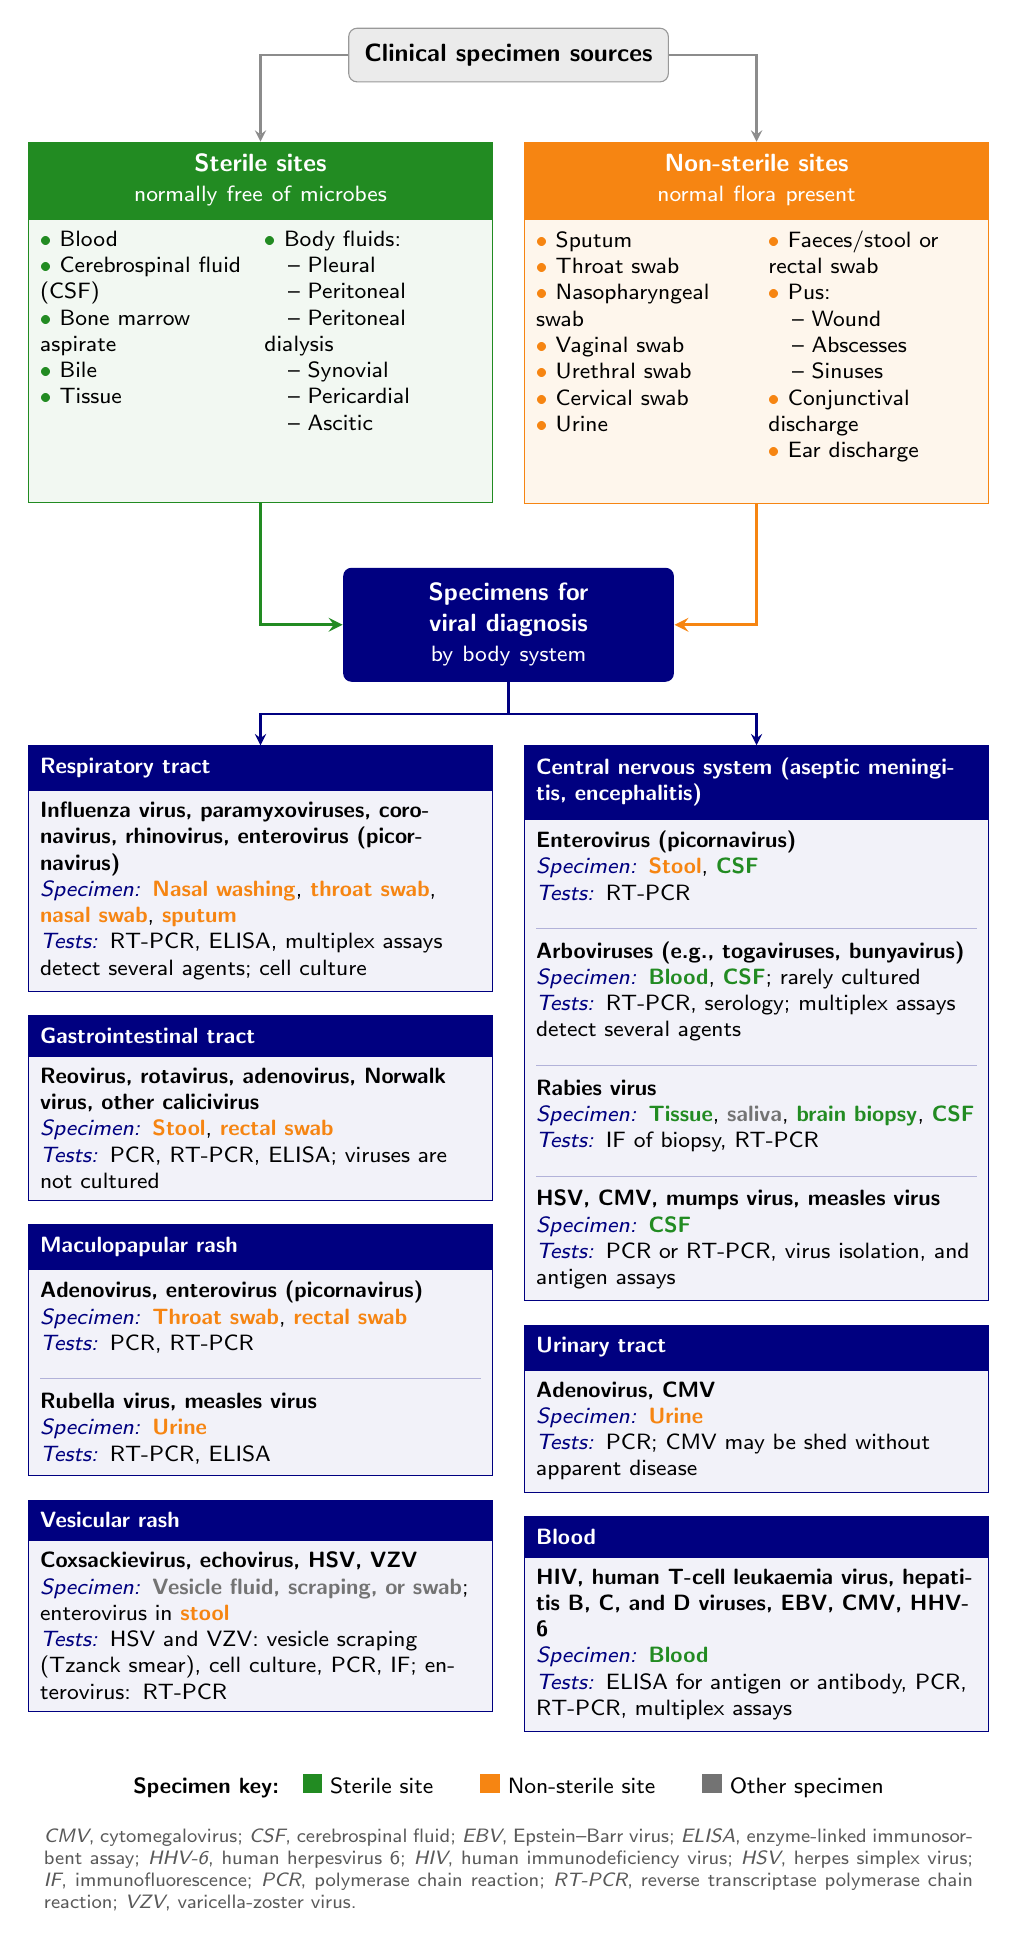
\begin{tikzpicture}[
      >=stealth,
      font=\sffamily,
      root/.style={draw=black!40, fill=black!8, rounded corners=3pt,
                   inner sep=2mm, font=\sffamily\bfseries\small},
      sterilehead/.style={draw=ForestGreen, fill=ForestGreen, text=white,
                   text width=5.6cm, align=center, inner sep=1.5mm,
                   font=\sffamily\bfseries\small},
      sterilebody/.style={draw=ForestGreen, fill=ForestGreen!6,
                   text width=5.6cm, align=left, inner sep=1.5mm,
                   font=\sffamily\footnotesize},
      nonsterilehead/.style={draw=BurntOrange, fill=BurntOrange, text=white,
                   text width=5.6cm, align=center, inner sep=1.5mm,
                   font=\sffamily\bfseries\small},
      nonsterilebody/.style={draw=BurntOrange, fill=BurntOrange!6,
                   text width=5.6cm, align=left, inner sep=1.5mm,
                   font=\sffamily\footnotesize},
      banner/.style={fill=NavyBlue, text=white, rounded corners=3pt,
                   text width=3.8cm, align=center, inner sep=2mm,
                   font=\sffamily\bfseries\small},
      cardhead/.style={draw=NavyBlue, fill=NavyBlue, text=white,
                   text width=5.6cm, align=left, inner sep=1.5mm,
                   font=\sffamily\bfseries\footnotesize},
      cardbody/.style={draw=NavyBlue, fill=NavyBlue!5,
                   text width=5.6cm, align=left, inner sep=1.5mm,
                   font=\sffamily\footnotesize},
    ]

    % ---------- Reference coordinates ----------
    \coordinate (O) at (0,0);
    \coordinate (L) at (-3.15,0);
    \coordinate (R) at (3.15,0);

    % ================= TOP: SPECIMEN SOURCES =================
    \node[root] (root) at (O) {Clinical specimen sources};

    % ---- Sterile sites ----
    \node[sterilehead, anchor=north] (st-h) at (-3.15,-1.1)
      {Sterile sites\\{\footnotesize\mdseries normally free of microbes}};
    \node[sterilebody, anchor=north] (st) at (st-h.south) {%
      \begin{minipage}[t][3.3cm][t]{2.75cm}\raggedright
        \textcolor{ForestGreen}{\textbullet}~Blood\\
        \textcolor{ForestGreen}{\textbullet}~Cerebrospinal fluid (CSF)\\
        \textcolor{ForestGreen}{\textbullet}~Bone marrow aspirate\\
        \textcolor{ForestGreen}{\textbullet}~Bile\\
        \textcolor{ForestGreen}{\textbullet}~Tissue
      \end{minipage}\hfill
      \begin{minipage}[t][3.3cm][t]{2.75cm}\raggedright
        \textcolor{ForestGreen}{\textbullet}~Body fluids:\\
        \hspace*{3mm}-- Pleural\\
        \hspace*{3mm}-- Peritoneal\\
        \hspace*{3mm}-- Peritoneal dialysis\\
        \hspace*{3mm}-- Synovial\\
        \hspace*{3mm}-- Pericardial\\
        \hspace*{3mm}-- Ascitic
      \end{minipage}};

    % ---- Non-sterile sites ----
    \node[nonsterilehead, anchor=north] (ns-h) at (3.15,-1.1)
      {Non-sterile sites\\{\footnotesize\mdseries normal flora present}};
    \node[nonsterilebody, anchor=north] (ns) at (ns-h.south) {%
      \begin{minipage}[t][3.3cm][t]{2.85cm}\raggedright
        \textcolor{BurntOrange}{\textbullet}~Sputum\\
        \textcolor{BurntOrange}{\textbullet}~Throat swab\\
        \textcolor{BurntOrange}{\textbullet}~Nasopharyngeal swab\\
        \textcolor{BurntOrange}{\textbullet}~Vaginal swab\\
        \textcolor{BurntOrange}{\textbullet}~Urethral swab\\
        \textcolor{BurntOrange}{\textbullet}~Cervical swab\\
        \textcolor{BurntOrange}{\textbullet}~Urine
      \end{minipage}\hfill
      \begin{minipage}[t][3.3cm][t]{2.65cm}\raggedright
        \textcolor{BurntOrange}{\textbullet}~Faeces/stool or rectal swab\\
        \textcolor{BurntOrange}{\textbullet}~Pus:\\
        \hspace*{3mm}-- Wound\\
        \hspace*{3mm}-- Abscesses\\
        \hspace*{3mm}-- Sinuses\\
        \textcolor{BurntOrange}{\textbullet}~Conjunctival discharge\\
        \textcolor{BurntOrange}{\textbullet}~Ear discharge
      \end{minipage}};

    \draw[->, thick, black!45] (root.west) -| (st-h.north);
    \draw[->, thick, black!45] (root.east) -| (ns-h.north);

    % ================= MIDDLE: BANNER =================
    \coordinate (topend) at (O |- current bounding box.south);
    \node[banner, anchor=north] (banner) at ([yshift=-8mm]topend)
      {Specimens for viral diagnosis\\{\footnotesize\mdseries by body system}};

    \draw[->, very thick, ForestGreen] (st.south) |- (banner.west);
    \draw[->, very thick, BurntOrange] (ns.south) |- (banner.east);

    \coordinate (cards) at ([yshift=-8mm]banner.south);
    \draw[->, thick, NavyBlue] (banner.south) -- ++(0,-4mm) -| (L |- cards);
    \draw[->, thick, NavyBlue] (banner.south) -- ++(0,-4mm) -| (R |- cards);

    % ================= LEFT COLUMN =================
    % ---- Respiratory tract ----
    \node[cardhead, anchor=north] (resp-h) at (L |- cards) {Respiratory tract};
    \node[cardbody, anchor=north] (resp) at (resp-h.south) {%
      \textbf{Influenza virus, paramyxoviruses, coronavirus, rhinovirus, enterovirus (picornavirus)}\\
      \textcolor{NavyBlue}{\textit{Specimen:}}
        \textcolor{BurntOrange}{\textbf{Nasal washing}}, \textcolor{BurntOrange}{\textbf{throat swab}},
        \textcolor{BurntOrange}{\textbf{nasal swab}}, \textcolor{BurntOrange}{\textbf{sputum}}\\
      \textcolor{NavyBlue}{\textit{Tests:}} RT-PCR, ELISA, multiplex assays detect several agents; cell culture};

    % ---- Gastrointestinal tract ----
    \node[cardhead, anchor=north] (gi-h) at ([yshift=-3mm]resp.south) {Gastrointestinal tract};
    \node[cardbody, anchor=north] (gi) at (gi-h.south) {%
      \textbf{Reovirus, rotavirus, adenovirus, Norwalk virus, other calicivirus}\\
      \textcolor{NavyBlue}{\textit{Specimen:}}
        \textcolor{BurntOrange}{\textbf{Stool}}, \textcolor{BurntOrange}{\textbf{rectal swab}}\\
      \textcolor{NavyBlue}{\textit{Tests:}} PCR, RT-PCR, ELISA; viruses are not cultured};

    % ---- Maculopapular rash ----
    \node[cardhead, anchor=north] (mac-h) at ([yshift=-3mm]gi.south) {Maculopapular rash};
    \node[cardbody, anchor=north] (mac) at (mac-h.south) {%
      \textbf{Adenovirus, enterovirus (picornavirus)}\\
      \textcolor{NavyBlue}{\textit{Specimen:}}
        \textcolor{BurntOrange}{\textbf{Throat swab}}, \textcolor{BurntOrange}{\textbf{rectal swab}}\\
      \textcolor{NavyBlue}{\textit{Tests:}} PCR, RT-PCR\\[1pt]
      {\color{NavyBlue!30}\rule{5.6cm}{0.4pt}}\\[1pt]
      \textbf{Rubella virus, measles virus}\\
      \textcolor{NavyBlue}{\textit{Specimen:}} \textcolor{BurntOrange}{\textbf{Urine}}\\
      \textcolor{NavyBlue}{\textit{Tests:}} RT-PCR, ELISA};

    % ---- Vesicular rash ----
    \node[cardhead, anchor=north] (ves-h) at ([yshift=-3mm]mac.south) {Vesicular rash};
    \node[cardbody, anchor=north] (ves) at (ves-h.south) {%
      \textbf{Coxsackievirus, echovirus, HSV, VZV}\\
      \textcolor{NavyBlue}{\textit{Specimen:}}
        \textcolor{black!55}{\textbf{Vesicle fluid, scraping, or swab}};
        enterovirus in \textcolor{BurntOrange}{\textbf{stool}}\\
      \textcolor{NavyBlue}{\textit{Tests:}} HSV and VZV: vesicle scraping (Tzanck smear),
        cell culture, PCR, IF; enterovirus: RT-PCR};

    % ================= RIGHT COLUMN =================
    % ---- Central nervous system ----
    \node[cardhead, anchor=north] (cns-h) at (R |- cards)
      {Central nervous system (aseptic meningitis, encephalitis)};
    \node[cardbody, anchor=north] (cns) at (cns-h.south) {%
      \textbf{Enterovirus (picornavirus)}\\
      \textcolor{NavyBlue}{\textit{Specimen:}}
        \textcolor{BurntOrange}{\textbf{Stool}}, \textcolor{ForestGreen}{\textbf{CSF}}\\
      \textcolor{NavyBlue}{\textit{Tests:}} RT-PCR\\[1pt]
      {\color{NavyBlue!30}\rule{5.6cm}{0.4pt}}\\[1pt]
      \textbf{Arboviruses (e.g., togaviruses, bunyavirus)}\\
      \textcolor{NavyBlue}{\textit{Specimen:}}
        \textcolor{ForestGreen}{\textbf{Blood}}, \textcolor{ForestGreen}{\textbf{CSF}}; rarely cultured\\
      \textcolor{NavyBlue}{\textit{Tests:}} RT-PCR, serology; multiplex assays detect several agents\\[1pt]
      {\color{NavyBlue!30}\rule{5.6cm}{0.4pt}}\\[1pt]
      \textbf{Rabies virus}\\
      \textcolor{NavyBlue}{\textit{Specimen:}}
        \textcolor{ForestGreen}{\textbf{Tissue}}, \textcolor{black!55}{\textbf{saliva}},
        \textcolor{ForestGreen}{\textbf{brain biopsy}}, \textcolor{ForestGreen}{\textbf{CSF}}\\
      \textcolor{NavyBlue}{\textit{Tests:}} IF of biopsy, RT-PCR\\[1pt]
      {\color{NavyBlue!30}\rule{5.6cm}{0.4pt}}\\[1pt]
      \textbf{HSV, CMV, mumps virus, measles virus}\\
      \textcolor{NavyBlue}{\textit{Specimen:}} \textcolor{ForestGreen}{\textbf{CSF}}\\
      \textcolor{NavyBlue}{\textit{Tests:}} PCR or RT-PCR, virus isolation, and antigen assays};

    % ---- Urinary tract ----
    \node[cardhead, anchor=north] (uri-h) at ([yshift=-3mm]cns.south) {Urinary tract};
    \node[cardbody, anchor=north] (uri) at (uri-h.south) {%
      \textbf{Adenovirus, CMV}\\
      \textcolor{NavyBlue}{\textit{Specimen:}} \textcolor{BurntOrange}{\textbf{Urine}}\\
      \textcolor{NavyBlue}{\textit{Tests:}} PCR; CMV may be shed without apparent disease};

    % ---- Blood ----
    \node[cardhead, anchor=north] (bld-h) at ([yshift=-3mm]uri.south) {Blood};
    \node[cardbody, anchor=north] (bld) at (bld-h.south) {%
      \textbf{HIV, human T-cell leukaemia virus, hepatitis B, C, and D viruses, EBV, CMV, HHV-6}\\
      \textcolor{NavyBlue}{\textit{Specimen:}} \textcolor{ForestGreen}{\textbf{Blood}}\\
      \textcolor{NavyBlue}{\textit{Tests:}} ELISA for antigen or antibody, PCR, RT-PCR, multiplex assays};

    % ================= LEGEND AND ABBREVIATIONS =================
    \coordinate (bottom) at (O |- current bounding box.south);
    \node[anchor=north, font=\sffamily\footnotesize] (legend) at ([yshift=-4mm]bottom) {%
      \textbf{Specimen key:}\quad
      \textcolor{ForestGreen}{\rule{2.5mm}{2.5mm}}~Sterile site\qquad
      \textcolor{BurntOrange}{\rule{2.5mm}{2.5mm}}~Non-sterile site\qquad
      \textcolor{black!55}{\rule{2.5mm}{2.5mm}}~Other specimen};
    \node[anchor=north, text width=11.8cm, align=justify,
          font=\sffamily\scriptsize, text=black!65] at ([yshift=-1.5mm]legend.south) {%
      \textit{CMV}, cytomegalovirus; \textit{CSF}, cerebrospinal fluid; \textit{EBV}, Epstein--Barr virus;
      \textit{ELISA}, enzyme-linked immunosorbent assay; \textit{HHV-6}, human herpesvirus 6;
      \textit{HIV}, human immunodeficiency virus; \textit{HSV}, herpes simplex virus;
      \textit{IF}, immunofluorescence; \textit{PCR}, polymerase chain reaction;
      \textit{RT-PCR}, reverse transcriptase polymerase chain reaction;
      \textit{VZV}, varicella-zoster virus.};

  \end{tikzpicture}%
  }
  \captionof{figure}[Specimen sources for viral diagnosis]{Clinical specimen sources (sterile vs.\ non-sterile) and specimens for viral diagnosis by body system. Specimens in the lower panels are colour-coded by site type.}
  \labfig{virus_sites}
\end{figure}

After a viral specimen has been collected, it must be placed into \textbf{viral transport medium}\index{viral transport medium}, which should be kept in a cold and moist environment (\textbf{but not frozen}). If the transit time is expected to exceed an hour, the container should also be sent with cold packs or ice.

Methods for the detection of viruses may be classified into either direct or indirect methods. \textbf{Direct methods}\index{viral identification!direct methods} refer to methods which directly sense the components of a virus. Examples include microscopic examination, viral culture, antigen detection or nucleic acid detection. \textbf{Indirect methods}\index{viral identification!indirect methods} are methods which detect antibodies in patient serum. They are alternatively referred to as \textbf{serological methods}\index{viral identification!serological methods}\index{serology|see{viral identification}}.

\section{Microscopy}
\index{virus!diagnosis!microscopy}

\textbf{Electron microscopy}\index{microscopy!electron} is a technique that may be used to directly visualise viruses. It allows for the determination of morphological features of a virus (size, shape, ultrastructural features). However, it is limited by sensitivity, as approximately 10\textsuperscript{6} particles per mL are required for accurate visualisation and identification. One technique to allow for easier detection of viruses is by addition of a virus-specific antibody, which clumps together viral particles to allow for easier visualisation. This is referred to as \textbf{immunoelectron microscopy}\index{microscopy!immunoelectron}.

\textbf{Light microscopy}\index{microscopy!light} is also used for the identification of viruses by analysis of viral proliferation within cell monolayers. This is achieved by the observation of morphologic changes in host cells following infection, often referred to as \textbf{cytopathology}\index{viral pathology!cytopathology}.\footnote{This includes pathology such as swelling/shrinking and syncytium (multinucleated cell) formation.} For instance, a Tzanck smear (see: Box~\ref{box:Tzanck-smear}) may be utilised in the detection of cutaneous disorders such as herpes or chickenpox.

\marginnote{\begin{kaobox}[frametitle={What is the Tzanck smear?},backgroundcolor=RoyalBlue!12!White,frametitlebackgroundcolor=RoyalBlue!25!White]\label{box:Tzanck-smear}
A \textbf{Tzanck smear}\index{Tzanck smear} is used in the detection of \textbf{acantholytic cells}\index{acantholytic cells},\footnote{Cells which have lost coherence because of disruption of intracellular bridges.} which tend to become rounded and present pathologic intraepidermal clefts, vesicles and bullae.
\end{kaobox}}

\section{Viral Culture}\label{sec:viral-culture}
\index{virus!diagnosis!culture}
\textbf{Viral culture}\index{viral culture} involves the isolation and cultivation of viruses within cells. One viral culture technique is the inoculation of the isolated virus into an \textbf{embryonated egg}\index{viral culture!embryonated egg} (specific parts depending on the virus suspected). In this technique, specimens are inoculated and incubation is performed for 2--9 days before harvest. Virus-infected eggs will show pocks or lesions within the cell membrane. Alternatively, viral culture is also performed in tissue cultures and cell lines. Viral culture may also be used in the determination of TCID\textsubscript{50}, LD\textsubscript{50} and ID\textsubscript{50}. Refer to Box~\ref{box:virus-property-infect} for details on each measure. The main preparations utilised for virus culture follow.

\begin{itemize}
  \item \textbf{Primary cell lines}\index{cell line!primary} --- consist of tissues that have been prepared from animal or human tissues (can be subcultured for relatively few passages).
  \item \textbf{Secondary cells}\index{cell line!secondary} --- tissue cells prepared from animal or human cells (can be subcultured approximately 20--50 times in vitro).
  \item \textbf{Continuous cell line}\index{cell line!continuous} --- cell lines derived from transformed or cancerous cells.
\end{itemize}

In addition to direct culture-based approaches to viral detection, we may also detect certain components or properties of a virus. Common methodologies for the detection of select viral properties follow.

\begin{itemize}
  \item The \textbf{plaque formation assay}\index{plaque formation assay}, which determines the number of plaque forming units (PFUs) in a cell culture by counting the number of discrete infectious centres (plaques formed by dead cells) within a volume of sample. The plaque forming assay is the gold standard for viral quantitation.
  \item The \textbf{haemagglutination test}\index{haemagglutination test} is a test used to detect the presence of viral antigens capable of causing red blood cell agglutination (haemagglutinin proteins) by adsorbing to the cells and subsequently forming a lattice. The reported value of this test is the greatest titre of virus which is still able to induce agglutination.
  \item \textbf{Detection of specific antigens}\index{antigen detection} may be performed to determine the presence of a suspected virus. Major methods include the \textbf{enzyme-linked immunosorbent assay (ELISA)}\index{ELISA}, latex particle agglutination, immunochromatography and immunostains\footnote{One example of this is immunoperoxidase staining, which allows for the detection of viral antigens by enzyme-conjugated antibodies.} (refer to Chapter~\ref{sec:immuno_diag} for an in-depth discussion of these techniques).
\end{itemize}

Genetic material may also be utilised to detect viruses. Common methods include:

\begin{itemize}
  \item The \textbf{Viral nucleic acid amplification test (NAAT)}\index{NAAT} utilises PCR (or qPCR) for the amplification of specific viral nucleic acid sequences. In \textbf{real-time PCR}\index{real-time PCR} (qPCR), fluorescent dye or labelled probes are utilised to identify the increase in genetic material induced by the amplification of nucleic acid sequences. Furthermore, qPCR may be utilised to detect the viral load of a sample.
  \item \textbf{Sanger sequencing}\index{Sanger sequencing} or chain-terminating PCR is an approach that allows for the sequencing of a given nucleic acid sequence by PCR with ddNTPs (fluorescent tagged chain-terminating dNTPs). We then filter fragments by size within a capillary, and detect the DNA base presented by fragments as they flow past.
  \item \textbf{Next-generation sequencing}\index{next-generation sequencing} refers to the simultaneous high-throughput sequencing of DNA or RNA fragments through a series of steps on a reaction cell. This approach utilises sequencing by synthesis.
\end{itemize}

\section{Serological Detection}
\index{virus!diagnosis!serology}
\index{virus!diagnostic tests!antibody tests}

The \textbf{serological methods}\index{viral identification!serological methods} of virus detection are an indirect approach to the detection of a virus. These methods detect the presence of virus-specific antibody within patient serum. Two main antibody types are tested for: IgM for acute infections\footnote{Though it often lacks specificity.} (as it appears early in the immune response), and IgG for the detection of immunity to a pathogen, or to diagnose a chronic infection.

Methods for the detection of antibodies include: enzyme immunoassay, radioimmunoassay, western blot, latex particle agglutination, viral neutralisation, haemagglutination inhibition, plaque reduction neutralisation, immunofluorescence, immunodiffusion and complement fixation. Refer to Chapter~\ref{sec:immuno_diag} for details.

\chapter{Poxviridae and Parvoviridae Species}
{}\margintoc{}

\section{Poxviridae}

The \textbf{Poxviridae}\index{Poxviridae} family are complex, enveloped dsDNA viruses (genome size 130--300 kbp). They are also known as the largest and most complex viruses. This family is historically known for their characteristic skin lesions (known as \textbf{pocks}\index{pocks}). Members of this family are shown in \reftab{c6-poxviridae-classification}.

\begin{table}[htbp]
  \centering
  \caption[Selected Poxviridae genera]{Classification of selected genera of the family Poxviridae, representative viruses, primary hosts, and associated diseases.}
  \labtab{c6-poxviridae-classification}
  \footnotesize
  \setlength{\tabcolsep}{2pt}
  \renewcommand{\arraystretch}{1.15}
  \begin{tabular}{@{}
    >{\RaggedRight\arraybackslash}p{0.16\textwidth}
    >{\RaggedRight\arraybackslash}p{0.22\textwidth}
    >{\RaggedRight\arraybackslash}p{0.18\textwidth}
    >{\RaggedRight\arraybackslash}p{0.39\textwidth}
    @{}}
    \toprule
    \textbf{Genus} &
    \textbf{Virus} &
    \textbf{Primary host} &
    \textbf{Disease} \\
    \midrule

    \multirow{4}{0.16\textwidth}{\centering\itshape Orthopoxvirus}
    & Variola
    & Humans
    & Smallpox (now eliminated) \\

    & Vaccinia
    & Humans
    & Localised lesion; used for smallpox vaccination \\

    & Mpox (Monkeypox) (Jan, 2022 outbreak)
    & Rodents, monkeys
    & Human infections rare; generalised disease \\

    & Cowpox
    & Cows
    & Human infections rare; localised ulcerating lesion \\

    \midrule

    \multirow{3}{0.16\textwidth}{\centering\itshape Parapoxvirus}
    & Orf
    & Sheep
    & \multirow{3}{0.39\textwidth}{\RaggedRight
      Human infections rare; localised lesion} \\

    & Pseudocowpox
    & Cows
    & \\

    & Bovine papular stomatitis
    & Cows
    & \\

    \midrule

    \multirow{1}{0.16\textwidth}{\centering\itshape Molluscipoxvirus}
    & Molluscum contagiosum
    & Humans
    & Many benign skin nodules \\

    \midrule

    \multirow{2}{0.16\textwidth}{\centering\itshape Yatapoxvirus}
    & Tanapox
    & Monkeys
    & Human infections rare; localised lesion \\

    & Yabapox
    & Monkeys
    & Human infections very rare and accidental;
      localised skin tumours \\

    \bottomrule
  \end{tabular}
\end{table}
  
The poxviruses are enveloped and brick/ovoid shaped viruses with a dumbbell core (where nucleic acids are stored) and lateral bodies. The virus also contains a DNA-dependent RNA polymerase which allows it to replicate within the cytoplasm, and it exists in two forms: an \textbf{extracellular enveloped virion (EEV)}\index{Poxviridae!extracellular enveloped virion (EEV)} and an \textbf{intracellular mature virion (IMV)}\index{Poxviridae!intracellular mature virion (IMV)}. The extracellular enveloped form is simply the IMV covered inside an envelope.

\subsection{Smallpox}

\textbf{Smallpox}\index{smallpox} (โรคฝีดาษ/ไข้ทรพิษ) is a disease caused by the Variola virus (a member of the Poxviridae family), and it was the first disease with a large-scale effective vaccination campaign. Smallpox is a human-specific virus (without an animal reservoir) with inhaled and cutaneous transmission. After infection, incubation is typically between 10 to 12 days (the range is between 7 to 17 days).

Two clinical forms of variola exist: Variola major and Variola minor. \textbf{Variola major}\index{smallpox!variola major} possesses a high fatality rate (30\%) and severity. It is the most common form of the virus worldwide. Meanwhile, \textbf{Variola minor}\index{smallpox!variola minor} is a less severe form with a 1--2\% mortality rate that only exists in some countries. Vaccines are available for smallpox. Signs and symptoms of smallpox include:

\begin{itemize}
  \item Prodromal symptoms: fever (of 38.3\textdegree{}C), severe headache, myalgia, fatigue, nausea and vomiting.
  \item Evolving rash initially appearing on the face and trunk, developing over 2--3 weeks with deep seated vesicles or pustules \textbf{at the same stage of development}, often with a centrifugal distribution\footnote{This means that lesions appear with the greatest concentration of lesions on the face and distal extremities.} (development process: macules \faArrowRight{} papules \faArrowRight{} vesicles \faArrowRight{} pustules \faArrowRight{} crusts).
\end{itemize}

The laboratory of smallpox requires BSL4, and includes NAAT as well as vesicle/fluid/scab samples.

One possible differential of smallpox is chickenpox, which also induces pox lesions, though clinical presentation differs. In chickenpox, lesions are more centrally distributed (with none on the palms or soles), rapidly developing and appear at the same time as fever. However, death from smallpox is relatively common (1 in 10) when compared to chickenpox.\footnote{Note that smallpox has been eradicated.}

\subsection{Mpox}

\textbf{Mpox}\index{mpox} is an infection caused by the monkeypox virus which resides in African rodents and monkeys. It may be transmitted to humans from these animals (by direct contact with body fluids/lesions of an infected animal), as well as between humans (by respiratory secretions, skin lesions or contaminated objects).

Signs and symptoms of Mpox typically resemble those of smallpox, albeit with reduced severity. Therefore, potential differential diagnoses for the rash include chickenpox, measles, bacterial skin infections, scabies, syphilis, and medication-associated allergies. The incubation period of Mpox is typically 6 to 13 days, though it can range from 5 to 21 days. The infection may be divided into invasion and skin eruption phases.

Signs and symptoms of the invasion phase are:

\begin{itemize}
  \item Rash (80.7\%) --- includes systemic (47.3\%), oral, genital (44.1\%) or other locations.
  \item Fever (59.1\%)
  \item Headache (31\%)
  \item Prodromal lymphadenopathy (29.1\%)\footnote{If lymphadenopathy appears we can eliminate differentials of chickenpox, measles and smallpox (as these present with no lymphadenopathy).}
  \item Myalgia (28.2\%)
\end{itemize}

In the eruptive phase (1 to 3 days after fever), firm, rubbery, well circumscribed and deep seated lesions (potentially with umbilication) appear. These lesions may be used in PCR for a diagnosis.

Two strains of Mpox exist. Central African clade (Clade I) with a mortality rate of 10\% and West African clade (Clade II) with a mortality rate of 1\%. Mpox is endemic in Central and western Africa (Benin, Cameroon, Congo, Gabon). The treatment for Mpox is \textbf{tecovirimat}\index{antiviral drugs!tecovirimat} or \textbf{brincidofovir}\index{antiviral drugs!brincidofovir}.

\subsection{Molluscum contagiosum}

\textit{Molluscum contagiosum}\index{molluscum contagiosum} is a viral infection of keratinocytes\index{keratinocytes} transmitted by direct contact (including sexual contact) and fomites. It has an incubation period between 2 weeks and 6 months, and is typically found in children and the immunocompromised. Following incubation, \textbf{Mollusca}\index{molluscum contagiosum!mollusca} appear.\footnote{Mollusca are small, firm, dome-shaped, pearly or flesh-coloured papules with central umbilication. They are painless and non-pruritic, typically presenting without inflammation.} Biopsy of these lesions may be considered in the presence of atypical lesions or uncertain diagnosis, and would show large intracytoplasmic inclusion bodies (Henderson--Patterson bodies\index{Henderson--Patterson bodies|see{molluscum contagiosum}}, \textbf{molluscum bodies}\index{molluscum contagiosum!molluscum bodies}) within keratinocytes.

Treatment is oral cimetidine, though the infection is typically self-resolving (typically within 6 to 12 months). Cryotherapy, laser therapy or curettage may also be considered for the removal of lesions.

\section{Parvoviridae}

The \textbf{Parvoviridae}\index{Parvoviridae} family are small (18--26 nm) ssDNA and non-enveloped icosahedral viruses. They are some of the smallest viruses. Of the Parvovirus family, the most clinically significant genus is the \emph{Erythrovirus}\index{Parvoviridae!Erythrovirus}, also known as Parvovirus B19, \textbf{erythema infectiosum}\index{erythema infectiosum}, or fifth disease\index{fifth disease|see{erythema infectiosum}}\footnote{As it is the 5\textsuperscript{th} most common exanthem.}. It is common in children between 5 and 15 (with F>M prevalence), and major manifestations are also most common in children.

Parvovirus B19\index{parvovirus B19} only infects the nucleus of erythroid progenitors, causing `dog-ear' cytoplasmic projections.\footnote{These progenitors are located in the bone marrow for adults, and liver for children.} This is because viral protein 1 attaches to Globoside or Gb4\index{parvovirus B19!receptor}, which is a blood group P-antigen (endocytosis is mediated by α5β1 integrins and Ku80 autoantigen). Transmission is primarily through the respiratory tract, but may also occur through blood transfusions.

Following the febrile prodrome (low fever, fatigue), erythema infectiosum typically presents clinically as an immune complex deposition disorder in addition to anaemia (ranging from mild to severe). In children, this can result in a `slapped cheek'\index{erythema infectiosum!slapped cheek appearance} appearance in combination with arthralgia, while in adults, it typically manifests as a more severe prodrome and isolated arthropathy without rash (typically lasting 1--3 weeks).

Diagnosis may be made with clinical features in addition to serological methods (such as anti-B19V IgM/IgG ELISA to VP1 and VP2) or PCR (B19 DNA). Treatment in children is typically not required, as it is self-limiting (1--2 weeks), and paracetamol or ibuprofen may be used if needed. Meanwhile, adults should rest and stop activities, and NSAIDs (such as aspirin, ibuprofen or naproxen sodium) may also be prescribed. Key populations of concern are:

\begin{itemize}
  \item Pregnant women --- it can induce hydrops fetalis\index{hydrops fetalis}, anaemia, cardiac failure or adverse fetal outcomes
  \item Immunocompromised patients --- it can cause pure red cell aplasia\index{pure red cell aplasia} \faArrowRight{} severe anaemia, which is resolved with passive immunisation.
  \item Anaemic patients --- \textbf{transient aplastic crisis}\index{transient aplastic crisis} (the inability to produce RBCs) causing pallor, weakness, and lethargy may occur (blood transfusion may be required).
\end{itemize}

\chapter{Hepatitis Viruses}
\margintoc{}

% ===================== hep-viruses : figure =====================
\begin{figure*}[p]
\centering
\begin{adjustbox}{width=\paperwidth, keepaspectratio}

\begingroup

% ===================== hep-viruses : local definitions =====================

% ---- colours ----
\definecolor{hepAcute}{HTML}{1E8449}
\definecolor{hepChronic}{HTML}{B03A2E}
\definecolor{hepCoinf}{HTML}{6C3483}
\definecolor{hepOther}{HTML}{1F618D}
\definecolor{hepSlate}{HTML}{2E4053}
\definecolor{hepAmber}{HTML}{AF601A}
\definecolor{hepTeal}{HTML}{117A65}
\colorlet{hepfld}{black}

% ---- helper macros ----
\newcommand{\hepfld}[1]{\par\vspace{2.2pt}\noindent{\color{hepfld}\bfseries #1:}\ }
\newcommand{\hepsect}[1]{\par\vspace{5pt}\noindent{\color{hepfld}\bfseries\small #1}\par
  \vspace{-1pt}\noindent{\color{hepfld}\rule{\linewidth}{0.6pt}}\par\vspace{1pt}}
\newcommand{\hepptitle}[1]{\noindent{\color{hepfld}\bfseries\large #1}\par\vspace{4pt}}
\newcommand{\heppos}{\textcolor{hepChronic}{\textbf{+}}}
\newcommand{\hepneg}{\textcolor{black!45}{$-$}}

% ---- column types ----
\newcolumntype{J}[1]{>{\raggedright\arraybackslash}p{#1}}
\newcolumntype{K}[1]{>{\centering\arraybackslash}p{#1}}

% ---- private bullet list ----
\newlist{heplist}{itemize}{1}
\setlist[heplist]{nosep, itemsep=1.5pt, leftmargin=1.1em,
  label={\color{hepfld}\textbullet}}

% ---- TikZ styles ----
\tikzset{
  hep-viruses/.style={font=\sffamily},
  hep setcol/.style={execute at begin node={\colorlet{hepfld}{#1!80!black}}},
  hep root/.style={draw=hepSlate, fill=hepSlate, text=white, rounded corners=6pt,
                   align=center, inner sep=9pt, text width=24cm, drop shadow},
  hep cat/.style={hep setcol=#1, draw=#1!80!black, fill=#1!15, text=#1!40!black,
                  line width=1.2pt, rounded corners=5pt, align=center,
                  inner sep=6pt, minimum height=2.3cm, drop shadow},
  hep vhead/.style={hep setcol=#1, draw=#1!80!black, fill=#1!80!black, text=white,
                    line width=1pt, text width=5.6cm, align=center, inner sep=2mm,
                    font=\sffamily\bfseries\large},
  hep vbody/.style={hep setcol=#1, draw=#1!80!black, fill=#1!5, line width=1pt,
                    text width=5.6cm, align=left, inner sep=2mm,
                    font=\sffamily\footnotesize},
  hep panel/.style={hep setcol=#1, draw=#1!80!black, fill=#1!4, line width=1pt,
                    rounded corners=4pt, align=left, inner sep=2mm,
                    font=\sffamily\footnotesize},
  hep conn/.style={draw=hepSlate!70, line width=1.1pt,
                   -{Stealth[length=3mm,width=2.2mm]}, rounded corners=4pt},
}

% ===================== end local definitions =====================

\begin{tikzpicture}[hep-viruses]
  % =============================== ROOT ================================
\node[hep root] (root) at (16,0)
 {{\LARGE\bfseries Viral Hepatitis: Hepatitis A--E \& Other Hepatitis Viruses}\\[4pt]
  {\normalsize Classified by natural history (acute / chronic / co-infection)
   $\rightarrow$ virology, virulence, pathogenesis, transmission,
   clinical differentiation, diagnosis \& treatment}};

% ============================ CATEGORIES =============================
\node[hep cat=hepAcute, text width=11.8cm] (acat) at (3.2,-3)
 {{\Large\bfseries ACUTE (self-limited)}\\[3pt]\small
  Enteric, faecal--oral; non-enveloped in stool; no carrier state in
  immunocompetent hosts\\ \emph{``Vowels (A, E) hit your bowels''}};
\node[hep cat=hepChronic, text width=11.8cm] (ccat) at (16,-3)
 {{\Large\bfseries CHRONIC (persistent)}\\[3pt]\small
  Parenteral / sexual / perinatal; enveloped; persistence $\rightarrow$
  cirrhosis \& hepatocellular carcinoma (HCC)};
\node[hep cat=hepCoinf, text width=5.6cm] (dcat) at (25.6,-3)
 {{\Large\bfseries CO-/SUPER-INFECTION}\\[3pt]\small
  Defective satellite virus; needs HBV (HBsAg) to propagate};
\node[hep cat=hepOther, text width=5.6cm] (ocat) at (32,-3)
 {{\Large\bfseries OTHER AGENTS}\\[3pt]\small
  Non-A--E ``hepatitis'' viruses \& systemic viruses causing hepatitis};

\foreach \hepcat in {acat,ccat,dcat,ocat}
  \draw[hep conn] (root.south) -- ++(0,-0.55) -| (\hepcat.north);

% ============================ HEADERS ================================
\node[hep vhead=hepAcute,   anchor=north] (havh) at (0,-6.6)
  {{\Large HAV}\\{\normalsize\mdseries Hepatitis A virus $\cdot$ RNA}};
\node[hep vhead=hepAcute,   anchor=north] (hevh) at (6.4,-6.6)
  {{\Large HEV}\\{\normalsize\mdseries Hepatitis E virus $\cdot$ RNA}};
\node[hep vhead=hepChronic, anchor=north] (hbvh) at (12.8,-6.6)
  {{\Large HBV}\\{\normalsize\mdseries Hepatitis B virus $\cdot$ DNA}};
\node[hep vhead=hepChronic, anchor=north] (hcvh) at (19.2,-6.6)
  {{\Large HCV}\\{\normalsize\mdseries Hepatitis C virus $\cdot$ RNA}};
\node[hep vhead=hepCoinf,   anchor=north] (hdvh) at (25.6,-6.6)
  {{\Large HDV}\\{\normalsize\mdseries Hepatitis D (delta) $\cdot$ RNA}};
\node[hep vhead=hepOther,   anchor=north] (othh) at (32,-6.6)
  {{\Large OTHERS}\\{\normalsize\mdseries Non-A--E \& systemic viruses}};

\draw[hep conn] (acat.south) -- ++(0,-0.5) -| (havh.north);
\draw[hep conn] (acat.south) -- ++(0,-0.5) -| (hevh.north);
\draw[hep conn] (ccat.south) -- ++(0,-0.5) -| (hbvh.north);
\draw[hep conn] (ccat.south) -- ++(0,-0.5) -| (hcvh.north);
\draw[hep conn] (dcat.south) -- (hdvh.north);
\draw[hep conn] (ocat.south) -- (othh.north);

% HDV depends on HBV
\draw[hepCoinf!80!black, dashed, line width=1.2pt, -{Stealth[length=3mm]}]
  ([xshift=-1.5cm]hdvh.north) to[out=160,in=20]
  node[pos=0.3, fill=white, inner sep=1.5pt, font=\sffamily\scriptsize\bfseries,
       text=hepCoinf!80!black] {needs HBsAg envelope}
  ([xshift=1.5cm]hbvh.north);

% ============================== HAV ==================================
\node[hep vbody=hepAcute, anchor=north] (hav) at (havh.south) {%
\hepfld{Family} \textit{Picornaviridae}, genus \textit{Hepatovirus}
\hepfld{Genome} (+)ssRNA, linear, $\sim$7.5\,kb; \textbf{naked} icosahedral capsid
 (quasi-enveloped ``eHAV'' in blood); single serotype
\hepfld{Virulence factors} Acid-, bile- and heat-stable capsid (survives stomach and
 environment); quasi-envelope shields from neutralising Ab; 3C/3ABC protease
 cleaves MAVS \& TRIF $\Rightarrow$ blunts interferon response
\hepfld{Transmission} \textbf{Faecal--oral}: contaminated water/food, raw shellfish,
 travel, day-care, outbreaks; MSM, PWID, homelessness
\hepfld{Incubation} 15--50\,d (mean $\sim$28\,d); stool shedding peaks 1--2\,wk
 \emph{before} jaundice (most infectious pre-symptomatically)
\hepfld{Pathogenesis} Not directly cytopathic; hepatocyte injury by CD8$^+$ T and NK
 cells; virions exit via bile $\rightarrow$ faeces
\hepfld{Clinical} Age-dependent: $<$6\,y mostly anicteric; adults: prodrome (fever,
 malaise, anorexia, nausea, RUQ pain) $\rightarrow$ jaundice, dark urine, pale
 stool, pruritus. Variants: cholestatic, relapsing. Fulminant $<$1\% (risk: age
 $>$50, pre-existing liver disease)
\hepfld{Chronicity} \textbf{Never}; no carrier state; lifelong immunity
\hepfld{Diagnosis} \textbf{IgM anti-HAV} = acute; IgG anti-HAV = past infection or
 vaccination
\hepfld{Treatment} Supportive; avoid alcohol \& hepatotoxins; transplant-centre
 referral if acute liver failure (ALF)
\hepfld{Prevention} Inactivated vaccine (2 doses, 0 and 6--12\,mo). PEP within 2\,wk
 of exposure: vaccine; add IG if $<$12\,mo, immunocompromised or chronic liver
 disease. Hand hygiene; inactivated by boiling and chlorine
\hepfld{Pearl} Commonest acute viral hepatitis worldwide; food handlers excluded
 until 7\,d after jaundice onset};

% ============================== HEV ==================================
\node[hep vbody=hepAcute, anchor=north] (hev) at (hevh.south) {%
\hepfld{Family} \textit{Hepeviridae} (\textit{Paslahepevirus balayani})
\hepfld{Genome} (+)ssRNA, linear, $\sim$7.2\,kb; naked (quasi-enveloped in blood);
 3 ORFs; genotypes (gt) 1--4 infect humans
\hepfld{Virulence factors} ORF2 capsid (main neutralising target); ORF3 drives
 quasi-enveloped egress; gt1 in pregnancy: high viral load + hormonal/immune
 shift $\Rightarrow$ severe disease
\hepfld{Transmission} \textbf{gt1/2}: waterborne faecal--oral epidemics (South Asia,
 Africa, floods, refugee camps). \textbf{gt3/4}: \textbf{zoonotic} --
 undercooked pork/liver, wild boar, deer, shellfish (Europe, USA, Japan); also
 transfusion, vertical
\hepfld{Incubation} 15--60\,d (mean $\sim$40\,d)
\hepfld{Pathogenesis} Mainly immune-mediated, as for HAV
\hepfld{Clinical} Acute icteric, often cholestatic hepatitis; young adults (gt1) or
 older men (gt3). \textbf{Pregnancy (3rd trimester, gt1): ALF, mortality up to
 20--25\%}, haemorrhage, fetal loss. Acute-on-chronic liver failure in cirrhosis
\hepfld{Chronicity} None if immunocompetent; \textbf{chronic ($>$3\,mo) in
 immunosuppressed} (SOT, HIV, chemotherapy; gt3) $\rightarrow$ rapid fibrosis
\hepfld{Extrahepatic} Guillain--Barr\'e, neuralgic amyotrophy, encephalitis,
 glomerulonephritis (MPGN), pancreatitis, thrombocytopenia
\hepfld{Diagnosis} IgM anti-HEV; \textbf{HEV RNA} (blood/stool) -- mandatory if
 immunosuppressed (serology unreliable)
\hepfld{Treatment} Supportive. Chronic: reduce immunosuppression $\rightarrow$
 ribavirin $\sim$3\,mo
\hepfld{Prevention} Safe water \& sanitation; cook pork thoroughly ($\geq$71\,\textdegree C);
 vaccine (HEV\,239) licensed only in China and a few other countries
\hepfld{Pearl} Test for HEV in ``seronegative'' hepatitis and suspected DILI};

% ============================== HBV ==================================
\node[hep vbody=hepChronic, anchor=north] (hbv) at (hbvh.south) {%
\hepfld{Family} \textit{Hepadnaviridae} (\textit{Orthohepadnavirus})
\hepfld{Genome} \textbf{Only DNA hepatitis virus}: partially dsDNA, relaxed-circular,
 $\sim$3.2\,kb; \textbf{enveloped}; replicates via pregenomic RNA using viral
 \textbf{reverse transcriptase}; nuclear \textbf{cccDNA} = persistence reservoir;
 genotypes A--J
\hepfld{Virulence factors} \textbf{HBsAg} (envelope; vast excess of subviral particles
 = immune decoy); \textbf{HBeAg} (secreted, tolerogenic; marks high replication
 \& infectivity); \textbf{HBx} (transactivator, inhibits p53 $\Rightarrow$
 oncogenic); \textbf{DNA integration} $\Rightarrow$ HCC even without cirrhosis;
 entry receptor NTCP
\hepfld{Transmission} Blood (PWID; needle-stick up to 30\% if source HBeAg$^+$),
 sexual, \textbf{perinatal} (dominant in endemic Asia/Africa), household;
 stable on surfaces $\geq$7\,d
\hepfld{Incubation} 30--180\,d (mean $\sim$75\,d)
\hepfld{Pathogenesis} Not directly cytopathic; injury by HBV-specific CD8$^+$ T cells;
 immune complexes $\Rightarrow$ extrahepatic disease
\hepfld{Clinical} Acute: serum-sickness-like prodrome (fever, arthralgia, urticaria)
 $\rightarrow$ jaundice; ALF $\sim$0.5--1\%. Chronic phases: HBeAg$^+$ infection
 (``immune-tolerant'') $\rightarrow$ HBeAg$^+$ hepatitis $\rightarrow$ HBeAg$^-$
 infection (inactive carrier) $\rightarrow$ HBeAg$^-$ hepatitis (pre-core mutant).
 Reactivation with immunosuppression (rituximab, chemo)
\hepfld{Chronicity} Inversely age-related: \textbf{$\sim$90\% perinatal}, 25--50\% at
 1--5\,y, $<$5\% adults
\hepfld{Complications} Cirrhosis, HCC, ALF
\hepfld{Extrahepatic} Polyarteritis nodosa, membranous GN (esp. children), MPGN,
 serum sickness, aplastic anaemia (rare)
\hepfld{Diagnosis} HBsAg, anti-HBc (IgM/total), anti-HBs, HBeAg/anti-HBe, HBV DNA,
 ALT; fibrosis staging (elastography, FIB-4) -- see serology table
\hepfld{Treatment} Acute: supportive (NA if severe/ALF). Chronic: \textbf{tenofovir
 (TDF/TAF) or entecavir} (high resistance barrier, usually long-term);
 peg-IFN-$\alpha$ 48\,wk (finite, selected). Goal: HBsAg loss (``functional
 cure'', rare). NA prophylaxis before immunosuppression in HBsAg$^+$ (and
 high-risk anti-HBc$^+$)
\hepfld{Prevention} Recombinant HBsAg vaccine (3 doses; anti-HBs $\geq$10\,mIU/mL =
 protected); birth dose $<$24\,h. Infant of HBsAg$^+$ mother: \textbf{vaccine +
 HBIG within 12\,h}; maternal TDF in 3rd trimester if DNA $>$200{,}000\,IU/mL
\hepfld{Pearl} Ground-glass hepatocytes (HBsAg in ER; orcein$^+$); HCC
 surveillance even without cirrhosis in high-risk carriers};

% ============================== HCV ==================================
\node[hep vbody=hepChronic, anchor=north] (hcv) at (hcvh.south) {%
\hepfld{Family} \textit{Flaviviridae} (\textit{Hepacivirus hominis})
\hepfld{Genome} (+)ssRNA, linear, $\sim$9.6\,kb; \textbf{enveloped}; circulates as
 lipo-viro-particle (ApoE/ApoB); 8 genotypes (gt1 commonest; gt3 $\Rightarrow$
 steatosis, faster fibrosis)
\hepfld{Virulence factors} Error-prone NS5B RdRp (no proofreading) $\Rightarrow$
 \textbf{quasispecies}; \textbf{E2 hypervariable region} $\Rightarrow$ antibody
 escape (hence no vaccine); NS3/4A protease cleaves MAVS \& TRIF $\Rightarrow$
 blocks IFN; core/NS5A $\Rightarrow$ steatosis, insulin resistance. Entry: CD81,
 SR-B1, claudin-1, occludin
\hepfld{Transmission} \textbf{Blood}: PWID (commonest), transfusion pre-1992, unsafe
 injections, dialysis, tattoos; needle-stick $\sim$1.8\%; sexual (low; higher in
 HIV$^+$ MSM); perinatal $\sim$5\%
\hepfld{Incubation} 2--26\,wk (mean $\sim$6--8\,wk)
\hepfld{Pathogenesis} Weak/exhausted T-cell response $\Rightarrow$ persistence;
 chronic immune-mediated inflammation; chronic B-cell stimulation $\Rightarrow$
 cryoglobulins, lymphoma
\hepfld{Clinical} Acute: $\sim$80\% asymptomatic; fluctuating ALT; ALF very rare.
 Fatigue is the commonest chronic symptom
\hepfld{Chronicity} \textbf{75--85\%} $\rightarrow$ cirrhosis 10--20\% over 20--30\,y
 $\rightarrow$ HCC 1--4\%/y once cirrhotic. Cofactors: alcohol, HIV, HBV, obesity
\hepfld{Extrahepatic} \textbf{Mixed cryoglobulinaemia} (purpura, arthralgia, low C4),
 MPGN, porphyria cutanea tarda, lichen planus, B-cell NHL, type 2 diabetes,
 thyroiditis, sicca
\hepfld{Diagnosis} Anti-HCV Ab (screen) $\rightarrow$ \textbf{HCV RNA} confirms viraemia
 (Ab persists after clearance/cure); RNA alone in early acute or immunosuppressed
\hepfld{Treatment} Pangenotypic DAAs: \textbf{sofosbuvir/velpatasvir} 12\,wk or
 \textbf{glecaprevir/pibrentasvir} 8\,wk; \textbf{SVR12 $>$95\% = cure}. Check
 HBsAg/anti-HBc first (HBV reactivation); reinfection possible; continue HCC
 surveillance if cirrhotic
\hepfld{Prevention} No vaccine; harm reduction (needle--syringe programmes, OAT),
 blood-donor screening; screen all adults $\geq$18\,y once \& every pregnancy
\hepfld{Pearl} Histology: portal lymphoid aggregates, bile-duct injury, steatosis};

% ============================== HDV ==================================
\node[hep vbody=hepCoinf, anchor=north] (hdv) at (hdvh.south) {%
\hepfld{Taxonomy} \textit{Kolmioviridae}, genus \textit{Deltavirus}
\hepfld{Genome} Circular ($-$)ssRNA, $\sim$1.7\,kb -- \textbf{smallest known human
 virus}; rod-like, self-cleaving \textbf{ribozyme}; host RNA pol\,II
 rolling-circle replication; one protein (HDAg, small \& large); 8 genotypes
\hepfld{Virulence factors} \textbf{Defective}: borrows the \textbf{HBsAg envelope}
 (enters via NTCP); large-HDAg \textbf{farnesylation} needed for assembly; direct
 cytopathic + immune injury; usually suppresses HBV replication
\hepfld{Transmission} As HBV: blood (PWID), sexual; perinatal rare. Endemic: Mongolia,
 Mediterranean, Central Asia, Central/West Africa, Amazon basin
\hepfld{Incubation} Co-infection as HBV; superinfection $\sim$2--8\,wk
\hepfld{Co-infection} HBV + HDV acquired together: acute (often biphasic ALT),
 \textbf{$\uparrow$ ALF risk}; $>$95\% clear both
\hepfld{Superinfection} HDV on a chronic HBV carrier: severe flare, \textbf{80--90\%
 chronic HDV} = \textbf{most severe chronic viral hepatitis}; cirrhosis in
 5--10\,y, $\uparrow$ HCC \& decompensation
\hepfld{Diagnosis} Screen \textbf{every HBsAg$^+$} with anti-HDV $\rightarrow$
 quantitative HDV RNA. IgM anti-HBc: $+$ in co-infection, $-$ in superinfection
\hepfld{Treatment} Peg-IFN-$\alpha$ $\geq$48\,wk (SVR $\sim$25\%); \textbf{bulevirtide}
 (NTCP entry inhibitor; EU-approved); lonafarnib (prenylation inhibitor,
 investigational). NAs do \emph{not} suppress HDV (treat HBV component only)
\hepfld{Prevention} \textbf{HBV vaccination prevents HDV}; carriers: avoid exposure
 (harm reduction, safer sex)
\hepfld{Pearl} Suspect in an HBsAg$^+$ patient with severe/progressive disease
 despite low HBV DNA};

% ============================== OTHERS ===============================
\node[hep vbody=hepOther, anchor=north] (oth) at (othh.south) {%
\hepsect{Other ``hepatitis'' viruses}
\hepfld{HGV / GBV-C} \textit{Pegivirus hominis} (Flaviviridae), (+)ssRNA;
 blood/sexual; lymphotropic, \textbf{not hepatotropic}, no proven disease;
 HIV co-infection linked to slower progression
\hepfld{TTV / SEN-V} \textit{Anelloviridae}, circular ssDNA; ubiquitous, no proven
 liver disease; TTV load used as marker of immunosuppression in transplant
\hepfld{``Hepatitis F''} Proposed, never confirmed
\hepfld{Non-A--E} ``Seronegative'' hepatitis: exclude mimics; can precede
 hepatitis-associated aplastic anaemia
\hepsect{Systemic viruses causing hepatitis}
\hepfld{EBV} Mononucleosis: pharyngitis, lymphadenopathy, splenomegaly, atypical
 lymphocytes; mild (often cholestatic) ALT rise; heterophile / VCA-IgM
\hepfld{CMV} Transplant, HIV, neonates; ``owl-eye'' inclusions; (val)ganciclovir
\hepfld{HSV-1/2} \textbf{ALF in pregnancy (3rd trimester) or immunosuppressed};
 fever, ALT/AST $\gg$1000, often \emph{anicteric}, leukopenia, rash in $<$50\%;
 \textbf{start empirical IV acyclovir}
\hepfld{VZV} Disseminated varicella/zoster in immunosuppressed; acyclovir
\hepfld{Adenovirus} Children, HSCT/SOT recipients; 2022 paediatric cluster
 (HAdV-41 + AAV2); cidofovir if severe
\hepfld{Yellow fever} \textit{Flavivirus}, \textit{Aedes} mosquito; jaundice +
 haemorrhage + renal failure; midzonal necrosis, \textbf{Councilman bodies};
 live attenuated vaccine
\hepfld{Others} Dengue, Ebola/Lassa, measles, rubella, parvovirus B19, HHV-6,
 enteroviruses (neonates), SARS-CoV-2};

% ======================= ROW 1 : REFERENCE TABLES =====================
\coordinate (B1) at ([yshift=-1cm]current bounding box.south);

\node[hep panel=hepSlate, anchor=north west, text width=14.2cm] (cmp) at (havh.west |- B1) {%
\hepptitle{At-a-glance comparison: hepatitis A--E}
{\renewcommand{\arraystretch}{1.25}\setlength{\tabcolsep}{3pt}
\rowcolors{2}{white}{hepfld!7}
\begin{tabular}{@{}J{2.2cm}*{5}{J{2.15cm}}@{}}
\rowcolor{hepfld!18}
\textbf{Feature} & \textbf{\color{hepAcute!80!black}HAV} & \textbf{\color{hepChronic!80!black}HBV}
 & \textbf{\color{hepChronic!80!black}HCV} & \textbf{\color{hepCoinf!80!black}HDV}
 & \textbf{\color{hepAcute!80!black}HEV}\\
\textbf{Family} & Picornaviridae & Hepadnaviridae & Flaviviridae & Kolmioviridae & Hepeviridae\\
\textbf{Genome} & (+)ssRNA, linear & partial dsDNA, circular & (+)ssRNA, linear
 & ($-$)ssRNA, circular & (+)ssRNA, linear\\
\textbf{Envelope} & No$^{*}$ & Yes & Yes & Yes (HBsAg) & No$^{*}$\\
\textbf{Main route} & Faecal--oral & Blood, sex, perinatal & Blood (PWID) & Blood, sex
 & Faecal--oral; zoonotic\\
\textbf{Incubation} & 2--6\,wk & 1--6\,mo & 2--26\,wk & As HBV; super 2--8\,wk & 2--9\,wk\\
\textbf{Chronicity} & Never & 90\% neonates; $<$5\% adults & 75--85\%
 & Co $<$5\%; super 80--90\% & Immuno\-suppressed only\\
\textbf{Fulminant} & Rare ($<$1\%) & $\sim$1\% & Very rare & High (co-infection)
 & Pregnancy (gt1)\\
\textbf{HCC risk} & No & Yes (direct + cirrhosis) & Yes (via cirrhosis)
 & Yes (rapid cirrhosis) & No\\
\textbf{Key test} & IgM anti-HAV & HBsAg, IgM anti-HBc, DNA & Anti-HCV $\rightarrow$ RNA
 & Anti-HDV $\rightarrow$ RNA & IgM anti-HEV, RNA\\
\textbf{Treatment} & Supportive & TDF/TAF, ETV, peg-IFN & DAAs (curative)
 & Peg-IFN, bulevirtide & Supportive; RBV if chronic\\
\textbf{Vaccine} & Yes (inactivated) & Yes (recombinant) & No & Via HBV vaccine
 & Limited (China)\\
\end{tabular}}
\par\vspace{3pt}{\scriptsize $^{*}$Quasi-enveloped (eHAV/eHEV) in blood, naked in stool.
 ETV entecavir; RBV ribavirin.}};

\node[hep panel=hepChronic, anchor=north west, text width=9.8cm] (ser) at ([xshift=6mm]cmp.north east) {%
\hepptitle{HBV serology interpretation}
{\renewcommand{\arraystretch}{1.3}\setlength{\tabcolsep}{3pt}
\rowcolors{2}{white}{hepfld!7}
\begin{tabular}{@{}J{2.9cm}*{5}{K{1.15cm}}@{}}
\rowcolor{hepfld!18}
\textbf{Pattern} & \textbf{HBsAg} & \textbf{HBeAg} & \textbf{\scriptsize IgM anti-HBc}
 & \textbf{\scriptsize Total anti-HBc} & \textbf{\scriptsize Anti-HBs}\\
Susceptible & \hepneg & \hepneg & \hepneg & \hepneg & \hepneg\\
Acute infection & \heppos & \heppos & \heppos & \heppos & \hepneg\\
Window period & \hepneg & \hepneg & \heppos & \heppos & \hepneg\\
Resolved (natural immunity) & \hepneg & \hepneg & \hepneg & \heppos & \heppos\\
Vaccinated & \hepneg & \hepneg & \hepneg & \hepneg & \heppos\\
Chronic, HBeAg$^+$ (high replication) & \heppos & \heppos & \hepneg & \heppos & \hepneg\\
Chronic, HBeAg$^-$ (inactive or pre-core mutant: check DNA) & \heppos & \hepneg & \hepneg & \heppos & \hepneg\\
Isolated anti-HBc (occult HBV, remote resolved, false $+$) & \hepneg & \hepneg & \hepneg & \heppos & \hepneg\\
\end{tabular}}
\par\vspace{3pt}{\scriptsize Chronic = HBsAg $>$6\,mo. Anti-HBs alone = vaccine
 immunity. IgM anti-HBc may reappear at low titre in flares. HBeAg$^+$ / high
 HBV DNA = highly infectious. HBsAg loss + anti-HBs = functional cure.}};

\node[hep panel=hepCoinf, anchor=north west, text width=11.6cm] (hdvt) at ([xshift=6mm]ser.north east) {%
\hepptitle{HDV: co-infection vs superinfection}
{\renewcommand{\arraystretch}{1.3}\setlength{\tabcolsep}{3pt}
\rowcolors{2}{white}{hepfld!7}
\begin{tabular}{@{}J{2.4cm}J{4.35cm}J{4.35cm}@{}}
\rowcolor{hepfld!18}
\textbf{Feature} & \textbf{Co-infection} & \textbf{Superinfection}\\
Setting & HBV and HDV acquired simultaneously & HDV acquired by a chronic HBsAg carrier\\
IgM anti-HBc & \textbf{Positive} & \textbf{Negative} (IgG anti-HBc$^+$)\\
HBsAg & Transient & Persistent\\
Anti-HDV & IgM, then low/transient IgG & High-titre, persistent IgM + IgG\\
Acute course & Often biphasic ALT; more severe than HBV alone & Severe flare in a
 known carrier (may mimic HBV reactivation)\\
ALF risk & $\uparrow$ vs HBV alone & $\uparrow\uparrow$\\
Chronic HDV & $<$5\% & \textbf{80--90\%}\\
Long-term & Usually full recovery & Cirrhosis in 5--10\,y, HCC, decompensation\\
\end{tabular}}
\par\vspace{3pt}{\scriptsize \textbf{Test for HDV:} every HBsAg$^+$ patient -- especially
 PWID, people from endemic regions, HIV/HCV co-infection, MSM, sex workers,
 unexplained flares or active disease with low HBV DNA.}};

% ======================= ROW 2 : CLINICAL PANELS ======================
\coordinate (B2) at ([yshift=-0.6cm]current bounding box.south);

\node[hep panel=hepAmber, anchor=north west, text width=11.85cm] (clin) at (havh.west |- B2) {%
\hepptitle{Differentiating Factors}
\begin{heplist}
\item \textbf{Travel, shellfish, day-care, outbreak} $\rightarrow$ HAV
 (HEV gt1 in South Asia/Africa)
\item \textbf{Undercooked pork/game, transplant recipient} $\rightarrow$ HEV gt3
\item \textbf{Pregnant + acute liver failure} $\rightarrow$ HEV (endemic areas),
 HSV (fever, anicteric, ALT $\gg$1000); also consider AFLP, HELLP
\item \textbf{PWID, tattoos, dialysis, transfusion pre-1992} $\rightarrow$ HCV
 $>$ HBV $\pm$ HDV
\item \textbf{Born in endemic region, sexual/household contact, MSM}
 $\rightarrow$ HBV
\item \textbf{Known HBV carrier with a flare} $\rightarrow$ HDV superinfection,
 HBV reactivation (rituximab, chemo, DAAs), HBeAg seroconversion flare, drugs,
 another virus
\item \textbf{Extrahepatic clues}: arthritis--urticaria prodrome or PAN
 $\rightarrow$ HBV; purpura + low C4 / cryoglobulins, PCT $\rightarrow$ HCV;
 Guillain--Barr\'e, brachial neuritis $\rightarrow$ HEV
\item \textbf{Pharyngitis, lymphadenopathy, splenomegaly, atypical lymphocytes}
 $\rightarrow$ EBV/CMV
\item \textbf{Non-viral mimics}: paracetamol (ALT often $>$3000), ischaemic
 hepatitis (rapid rise/fall, high LDH), autoimmune hepatitis (IgG$\uparrow$,
 ANA/ASMA), Wilson disease ($<$40\,y, haemolysis, low ALP), alcohol (AST:ALT
 $>$2, AST rarely $>$300--400), DILI, biliary obstruction, Budd--Chiari
\end{heplist}};

\node[hep panel=hepOther, anchor=north west, text width=11.85cm] (labs) at ([xshift=6mm]clin.north east) {%
\hepptitle{Labs, severity, histopathology \& follow-up}
\begin{heplist}
\item \textbf{Acute viral pattern}: ALT $>$ AST, 10--100$\times$ ULN (often
 $>$1000\,IU/L); conjugated hyperbilirubinaemia; ALP mildly $\uparrow$
\item \textbf{Severity}: INR/PT is the best early prognostic marker (not the ALT
 level). \textbf{ALF} = INR $\geq$1.5 + encephalopathy, no prior liver disease,
 illness $<$26\,wk $\Rightarrow$ ICU and early transplant-centre referral
 (King's College criteria); NAC may help in early-grade non-paracetamol ALF
\item \textbf{Chronic}: HBsAg or viraemia $>$6\,mo; stage fibrosis
 non-invasively (APRI, FIB-4, transient elastography); biopsy if unclear
\item \textbf{Histology (acute)}: ballooning degeneration, acidophil
 (\textbf{Councilman}) bodies, lobular inflammation, cholestasis; bridging
 necrosis if severe
\item \textbf{Histology (specific)}: HBV ground-glass hepatocytes (HBsAg) \&
 ``sanded'' nuclei (HBcAg); HCV portal lymphoid aggregates, bile-duct injury,
 steatosis; chronic: interface hepatitis $\rightarrow$ bridging fibrosis
 $\rightarrow$ cirrhosis; HSV Cowdry A inclusions; CMV owl-eye inclusions;
 yellow fever midzonal (zone 2) necrosis
\item \textbf{Surveillance}: ultrasound $\pm$ AFP every 6\,mo in cirrhosis (any
 cause) and high-risk HBV carriers without cirrhosis (Asian men $>$40\,y, women
 $>$50\,y, African origin, family history of HCC); variceal screening if cirrhotic
\end{heplist}};

\node[hep panel=hepTeal, anchor=north west, text width=11.85cm] (prev) at ([xshift=6mm]labs.north east) {%
\hepptitle{Prevention, exposures, screening \& mnemonics}
\begin{heplist}
\item \textbf{Needle-stick risk (``rule of 3'')}: HBV $\sim$30\% (HBeAg$^+$
 source) $>$ HCV $\sim$3\% (actual $\sim$1.8\%) $>$ HIV $\sim$0.3\%
\item \textbf{PEP}: HBV -- unvaccinated/non-responder: HBIG + vaccine ASAP
 (ideally $\leq$24\,h, up to 7\,d); known responder: none. HCV -- no PEP: test
 source + baseline, HCV RNA at 3--6\,wk, treat if infected. HAV -- vaccine
 $\pm$ IG within 2\,wk
\item \textbf{Screening (CDC)}: HCV -- all adults $\geq$18\,y once + every
 pregnancy; HBV -- all adults $\geq$18\,y once (HBsAg, anti-HBs, total
 anti-HBc) + every pregnancy; HDV -- all HBsAg$^+$
\item \textbf{Vaccination}: HBV birth dose $<$24\,h + universal series; HAV
 universal childhood + travellers, MSM, PWID, homeless; both HAV and HBV for anyone
 with chronic liver disease
\item \textbf{Co-infection}: test HIV in all HBV/HCV (and vice versa); HIV/HBV
 $\Rightarrow$ tenofovir-based ART; stopping an NA can trigger a severe HBV flare
\item \textbf{Public health}: acute hepatitis A--E is notifiable; trace and
 vaccinate contacts
\item \textbf{Mnemonics}: ``\emph{Vowels hit your bowels}'' (A, E: enteric, not
 chronic); \textbf{B} = Blood, Birth, Bed (sex); \textbf{C} = Chronic, Cirrhosis,
 Carcinoma, Cryoglobulins; \textbf{D} = Defective, Dependent on B; \textbf{E} =
 Enteric, Expectant mothers, Eating pork
\end{heplist}};

% ============================== FOOTER ===============================
\coordinate (B3) at ([yshift=-0.5cm]current bounding box.south);
\node[anchor=north west, text width=37.6cm, align=left, inner sep=2mm,
      font=\sffamily\scriptsize, text=black!75] at (havh.west |- B3) {%
\textbf{Abbreviations:} AFLP acute fatty liver of pregnancy; AFP alpha-fetoprotein;
ALF acute liver failure; ANA/ASMA antinuclear/anti-smooth-muscle Ab; ART antiretroviral
therapy; DAA direct-acting antiviral; DILI drug-induced liver injury; GN
glomerulonephritis; gt genotype; HBIG hepatitis B immune globulin; HCC hepatocellular
carcinoma; HSCT haematopoietic stem-cell transplant; IG immune globulin; MPGN
membranoproliferative GN; MSM men who have sex with men; NA nucleos(t)ide analogue; NAC
N-acetylcysteine; NHL non-Hodgkin lymphoma; NTCP sodium taurocholate co-transporting
polypeptide; OAT opioid agonist therapy; PAN polyarteritis nodosa; PCT porphyria cutanea
tarda; PEP post-exposure prophylaxis; PWID people who inject drugs; RdRp RNA-dependent RNA
polymerase; RUQ right upper quadrant; SOT solid-organ transplant; SVR12 sustained
virological response 12\,wk post-treatment; TDF/TAF tenofovir disoproxil/alafenamide;
ULN upper limit of normal.\quad
\textit{Educational summary -- verify doses and current guidance (AASLD, EASL, WHO, CDC)
before clinical use.}};

\end{tikzpicture}

\endgroup

\end{adjustbox}
\caption[Viral hepatitis overview]{Viral hepatitis A--E and other hepatitis viruses: classification by natural history, virology, virulence, pathogenesis, transmission, diagnosis and treatment.}
\labfig{hep-viruses}
\end{figure*}
% =================== end hep-viruses figure ===================

\textbf{Hepatitis}\index{hepatitis} is defined as inflammation of the liver, which may be caused by a wide variety of viral and non-infectious agents. Clinical signs and symptoms include both prodromal signs (in infectious aetiology) and specific signs, including icterus.\footnote{These signs are caused by liver damage and include jaundice, dark urine and increased AST and ALT levels.} A summary of the hepatitis viruses is given in \reffig{hep-viruses}.

\section{Hepatitis A Virus}

The Hepatitis A virus\index{hepatitis A virus}\index{HAV|see{hepatitis A virus}} is a non-enveloped ssRNA+ strand virus transmitted primarily by the faecal-oral route.\footnote{Though it is non-enveloped, it exists in a \textbf{quasi-enveloped}\index{quasi-enveloped virion} form in the body to prevent immune detection.} It is a non-cytolytic virus able to induce exocytosis to the biliary system and subsequent faecal shedding. Consequently, risk factors include poor sanitation, close contact with infected individuals, use of recreational drugs and limited access to safe water.\footnote{MSM is also a risk factor for infection.} Over 90\% of the adult population is seropositive in developing countries.

Prevention is achieved by hygienic practices, avoidance of contaminated foods and chlorination of water. Additionally, \textbf{immune serum globulin}\index{immunoglobulin!hepatitis A} and a vaccine (covering Hepatitis A and B strains) are also available as preventative measures. The vaccine is recommended as \textbf{post-exposure prophylaxis}\index{prophylaxis!post-exposure} and for high-risk travellers.

Viral infection begins as the virus crosses the intestinal barrier and travels to the liver, where it establishes an infection within hepatocytes and subsequently produces progeny to be released into the bile (and subsequently the stool, which marks the infectious phase). The typical incubation period ranges from 3--6 weeks (average 4) and complete recovery typically occurs at 2--4 weeks following onset. Symptoms are typically minor in children, though adults may be symptomatic. Additionally, \textbf{fulminant hepatitis}\index{fulminant hepatitis} may occur. The virus is detectable both from symptoms and serology, with acute infections resulting in a + result of the IgM Anti-HAV screen (chronic/past infections will be positive for IgG).

Treatment of Hepatitis A is primarily supportive, with fluid replacement, nutrition and rest, as no specific antivirals are available. However, liver transplants may be considered in fulminant liver failure.

\section{Hepatitis B Virus}

The Hepatitis B virus\index{hepatitis B virus}\index{HBV|see{hepatitis B virus}} is an enveloped dsDNA virus that causes serum hepatitis. Transmission is through sexual contact, blood or vertical transmission,\footnote{HBs and HBe antigen presence in the mother indicate increased risk of transmission to the fetus.} with infectious materials being semen, vaginal secretions, contaminated blood, blood products and sharps. HBV may be prevented by the modification of risk behaviours and passive\footnote{Primarily for children born to infected mothers.}/active immunisation.

After entry of the virus into the bloodstream, it establishes an infection within the liver, causing damage to hepatocytes (ground glass hepatocyte pathology\index{hepatitis B virus!ground glass hepatocytes}). During the replication process, both \textbf{Dane particles}\index{hepatitis B virus!Dane particles} (infective particles) and `decoy' particles\index{hepatitis B virus!decoy particles} are released. Major antigens and antibodies of the virus follow.

\begin{itemize}
  \item \textbf{HBsAg}\index{hepatitis B virus!surface antigen (HBsAg)}\index{HBsAg|see{hepatitis B virus, surface antigen}} --- the Hepatitis B surface antigen,\footnote{Also known as the Australia antigen.} which indicates the presence of Hepatitis B infection. Presence of antibody to the HBs antigen indicates immunity to hepatitis B (either from past infections or vaccination).
  \item \textbf{HBcAg}\index{hepatitis B virus!core antigen (HBcAg)}\index{HBcAg|see{hepatitis B virus, core antigen}} --- the Hepatitis B core antigen, which is undetectable in serum. Presence of an antibody against this antigen is a clear marker of infection (IgM suggests recent infection, IgG suggests chronic or resolved infection).
  \item \textbf{HBeAg}\index{hepatitis B virus!e antigen (HBeAg)}\index{HBeAg|see{hepatitis B virus, e antigen}} --- the Hepatitis B nucleocapsid antigen, which is released by hepatocytes during active viral replication and indicates high transmissibility and a poor prognosis. An antibody to this antigen indicates lower transmissibility.
\end{itemize}

The incubation period of Hepatitis B is between 6--24 weeks (typically 2--3 months). Infection results in a prodromal phase \faArrowRight{} icteric phase \faArrowRight{} convalescent/fulminant phase (depending on host immune status). The chronic persistent presentation of Hepatitis B is often asymptomatic, while the chronic active presentation is typically more severe, and consequently more likely to induce hepatocellular carcinoma or cirrhosis.

Outcomes of HBV infection include acute disease with resolution in patients with effective cell-mediated immune responses, or chronic, mildly symptomatic disease in immunodeficiency. In chronic infection, fulminant hepatitis, hepatocellular carcinoma or cirrhosis may occur. There is no specific treatment in acute infection, though \textbf{interferons}\index{antiviral drugs!interferon}, \textbf{nucleosides}\index{antiviral drugs!nucleoside and nucleotide analogues} (nucleotide analogues, RT inhibitors) may be considered in chronic infection.

\section{Hepatitis C Virus}\label{HCV_thing}

\textbf{Hepatitis C}\index{hepatitis C virus}\index{HCV|see{hepatitis C virus}}, also known as post-transfusional non-A non-B hepatitis, is a spherical enveloped ssRNA+ virus. Notably, it lacks 3'-5' exonuclease, which causes it to be susceptible to mutations. Genotype 3 is common in Southeast Asia. It is composed of 3 structural proteins (C=core, E1 and E2) and 6 non-structural proteins (NS2, NS3, NS4A, NS4B, NS5A, NS5B). Many of these proteins are targeted by antiviral drugs, including:

\begin{itemize}
  \item \textbf{NS3/4A}\index{hepatitis C virus!NS3/4A protease}, which acts as a HCV protease.
  \item \textbf{NS5A}\index{hepatitis C virus!NS5A}, a phosphoprotein for replication and assembly.
  \item \textbf{NS5B}\index{hepatitis C virus!NS5B}, an RNA-dependent RNA polymerase.
\end{itemize}

Hepatitis C is primarily transmitted through blood, though it may rarely spread through sexual contact or vertical transmission. Therefore, prevention is through the screening of blood donors and medical precautions. It is typically a persistent infection.\footnote{A memory technique is: A for acute infections, B for `bad blood', C for chronic, and D for defective.} This is because HCV produces proteins which inhibit apoptosis and interferon alpha, promoting persistence. Damage from the infection is caused by cell-mediated immunity and immune complex deposition of anti-HCV antibodies within the liver and extrahepatic tissues (including vessels, joint spaces and kidneys). Diagnosis of Hepatitis C is made by the presence of anti-HCV antibody, antigen ELISA and PCR. However, these techniques do not differentiate between acute and chronic infection. Treatment of Hepatitis C differs between subgroups, but the typical regimens are:

\begin{itemize}
  \item \textbf{Direct-acting antivirals}\index{antiviral drugs!direct-acting antivirals}.
  \item \textbf{Pegylated interferon}\index{antiviral drugs!pegylated interferon}, potentially with \textbf{ribavirin}\index{antiviral drugs!ribavirin}.
  \item Liver transplantation for complicated infection.
\end{itemize}

\section{Hepatitis D Virus}

The Hepatitis D virus\index{hepatitis D virus}\index{HDV|see{hepatitis D virus}} is a defective enveloped ssRNA virus only capable of replicating in HBV-infected cells. Two mechanisms of infection exist for HDV: (1) \textbf{co-infection}\index{hepatitis D virus!co-infection} with HBV on the naive host, which presents with a higher severity and risk of fulminant hepatitis and (2) \textbf{superinfection}\index{hepatitis D virus!superinfection}, which is the infection of a HBV carrier.\footnote{The superinfection form is more severe, and presents a higher risk of developing hepatocellular carcinoma or cirrhosis.} Diagnosis of HDV is made by HDV IgM presence in addition to clinical symptoms. Treatment is by interferon alpha\index{antiviral drugs!interferon}, as nucleosides are ineffective.

\section{Hepatitis E Virus}

The Hepatitis E virus\index{hepatitis E virus}\index{HEV|see{hepatitis E virus}} is a ssRNA+ enteric water-borne virus. It is transmitted by the faecal-oral route from contaminated drinking water. It has 4 major genotypes with variable characteristics. Risk factors include pets, undercooked organ meat, infected cow's milk, swine, poor sanitation and lack of safe water. Prevention involves improving sanitation and food handling. Pathogenesis is similar to the Hepatitis A virus, with a 15--60-day (typically 40-day) incubation. It typically manifests as icteric (age 15--40 years) signs or anaemia in younger patients. Diagnosis is made by anti-HEV IgM, in addition to detection of the virus in stool or liver. Treatment is supportive, but ribavirin\index{antiviral drugs!ribavirin} may be used in persistent or severe infections.


\chapter{Central Nervous System Infections}
\margintoc{}

The \textbf{neurotropic viruses}\index{neurotropic} are a group of viruses that possess a selective affinity for nervous tissue. They may enter into the brain through many routes, including across the blood-brain barrier, through peripheral nerves (such as rabies) and through disrupted epithelium. They may cause many diseases, ranging from inflammation to death through a variety of mechanisms, including neuronal death, impairment of neurogenesis and immune dysfunction.

\section{The Poliovirus}

The Poliovirus\index{poliovirus} is a linear non-enveloped ssRNA+ virus only infecting humans (there are 3 serotypes of Polio). It is acid stable but susceptible to heat, formaldehyde, chlorine and UV light. Presently, it is nearly eradicated, with few risk regions remaining. \textbf{Transmission} is primarily through the faecal-oral route, though transmission through oral contact, food or water is also possible. Polio possesses a number of viral proteins, both structural and non-structural:

\begin{itemize}
  \item Surface proteins\index{poliovirus!surface proteins}:
  \begin{itemize}
    \item VP1 --- outer surface protein (on vertices) responsible for CD155 receptor binding and injection of RNA into the host cell.
    \item VP2 --- outer surface protein for structural integrity.
    \item VP3 --- capsid shell and icosahedral shape.
    \item VP4 --- inner surface protein stabilising genome, released during cell entry.
  \end{itemize}
  \item Viral replication proteins\index{poliovirus!replication proteins}:
  \begin{itemize}
    \item 2A (Pro) --- cleavage of eIF4G (host cell protein), causes shutdown of host protein synthesis.
    \item 2B --- viroporin, inhibits protein secretion and membrane permeability of host cell. Causes cell lysis.
    \item VPg (3B) --- linked to viral genome, acts as primer for RNA synthesis.
    \item 2C --- ATPase/helicase that anchors the replication complex to the host membrane and helps in RNA synthesis.
    \item 3D (Pol) --- RNA-dependent RNA polymerase.
  \end{itemize}
  \item Other proteins:
  \begin{itemize}
    \item VP0 --- precursor protein of VP2 and VP4.
    \item 3A --- inhibits protein trafficking and presentation of MHC type I (immune evasion).
  \end{itemize}
\end{itemize}

The Poliovirus\index{poliovirus} is transmitted by the faecal-oral route and enters epithelial cells by binding with the \textbf{CD155 receptor}\index{poliovirus!CD155 receptor}. It subsequently replicates in Peyer's patches\index{Peyer's patches} of the GI tract, and spreads to the CNS by retrograde axonal transport or viraemia to the anterior horn cells of the spinal cord and brainstem motor nuclei, leading to paralysis. Outcomes of the infection include asymptomatic infection (90\%), \textbf{abortive poliomyelitis}\index{poliomyelitis!abortive} with flu-like symptoms (5\%), \textbf{non-paralytic poliomyelitis}\index{poliomyelitis!non-paralytic}/aseptic meningitis, \textbf{paralytic poliomyelitis}\index{poliomyelitis!paralytic} (1\%) or \textbf{bulbar polio}\index{poliomyelitis!bulbar} (dysphagia, speech impairment).

Diagnosis is made by viral isolation from the stool or CSF (gold standard), though serology and PCR are often performed. Control mechanisms include vaccination (\textbf{inactivated polio vaccine}\index{polio vaccine!inactivated} \faArrowRight{} IgG, \textbf{oral polio vaccine}\index{polio vaccine!oral} \faArrowRight{} secretory IgA) and improved sanitation.

\section{Rabies}

The Rabies virus\index{rabies virus} is a linear ssRNA$-$ enveloped virus and a member of the \textit{Lyssavirus}\index{Lyssavirus} genus. It is able to infect all warm-blooded mammals, and is typically transmitted through the saliva of infected animals. It exists in two main forms: the \textbf{street strain}\index{rabies virus!street strain} and the \textbf{vaccine strain}\index{rabies virus!vaccine strain}. The spike glycoprotein (G) allows the virus to attach to host cells possessing the nicotinic acetylcholine receptor\index{nicotinic acetylcholine receptor} (nAChR)\index{nAChR|see{nicotinic acetylcholine receptor}}. Both strains infect the cytoplasm of neurons. In the street strain, this induces the formation of \textbf{Negri bodies}\index{Negri bodies}.\footnote{Described as eosinophilic, cytoplasmic inclusions found in neurons, most notably in the Purkinje cells.} However, the vaccine strain is less virulent, with lower neuroinvasiveness and wider dissemination without the generation of Negri bodies. Key structural proteins of the Rabies virus\index{rabies virus!structural proteins} are:

\begin{itemize}
  \item Nucleoprotein --- binds to the viral RNA and forms the nucleocapsid.
  \item Phosphoprotein --- RNA synthesis and replication.
  \item Matrix protein --- assembly and budding of virus.
  \item Glycoprotein --- viral attachment and entry to host cells.
  \item RNA-dependent RNA polymerase --- RNA replication, transcription.
\end{itemize}

The prevention of rabies includes avoidance, animal control in addition to \textbf{pre-exposure prophylaxis}\index{prophylaxis!pre-exposure} (2-dose series) and \textbf{post-exposure prophylaxis}\index{prophylaxis!post-exposure} (immunoglobulin\index{immunoglobulin!rabies}\footnote{Available in either human immunoglobulin or equine immunoglobulin forms. The immunoglobulin is only administered for wounds with bleeding/on broken skin, but vaccine is given for all exposures.} around the wound and vaccine).

Rabies initially replicates at the site of infection within muscle tissue\footnote{Modifying factors for infection risk include: wound location, severity of the injury and type of exposure.} (potentially for years) before binding to nAChRs and entering peripheral nerves. The virus then spreads in a retrograde manner by axonal transport to the CNS (dorsal root ganglion, spine, brain), where it causes neuronal dysfunction. Additionally, the virus resides in the salivary glands, which enables infected animals to propagate the virus. During the infection, symptoms\index{rabies virus!clinical features} begin with a non-specific prodrome which is followed by agitation, hyperexcitability, hydrophobia\index{rabies virus!hydrophobia}, aerophobia, autonomic dysfunction (potentially ascending paralysis instead if paralytic rabies) and eventually death within 7--10 days of symptom onset.

Diagnostic tests\index{rabies virus!diagnosis} include PCR of CSF or saliva, as well as \textbf{direct fluorescent antibody testing}\index{direct fluorescent antibody test} on neck skin biopsy. Post-mortem examination often finds Negri bodies\index{Negri bodies} in brain tissue. Additionally, cultures may be performed in cell lines or mice.

\chapter{Oncoviruses}
\margintoc{}

\textbf{Oncogenesis}\index{oncogenesis} refers to the process that transforms normal cells into cancer cells. This includes both genetic and epigenetic alterations that disrupt the balance between proliferation and apoptosis. One component of this process is the transformation of \textbf{proto-oncogenes}\index{proto-oncogene}\footnote{Positive regulators such as growth factors, hormones, ATP and phosphorylation.} and \textbf{anti-oncogenes}\index{tumour suppressor gene}\index{anti-oncogene|see{tumour suppressor gene}}\footnote{Examples include: tumour suppressor genes such as p53\index{tumour suppressor gene!p53} or pRB\index{tumour suppressor gene!pRB}.} (both major components that regulate the cell cycle and cell proliferation) into \textbf{oncogenes}\index{oncogene} which induce uncontrolled proliferation. This occurs either through loss-of-function\index{mutation!loss-of-function} mutations or gain-of-function\index{mutation!gain-of-function} mutations. Some potential mutations include: (1) translocation or transposition, leading to increased production as a result of a promoter; (2) increased gene amplification or (3) point mutations within the control element or gene that result in increased production or a hyperactive/degradation-resistant product.

As a result of many combined mutations (potentially as a combined result of genetic predisposition and environmental factors), cells may become immortal; this is referred to as \textbf{transformation}\index{oncogenesis!transformation}, which results in either a benign\index{tumour!benign} or malignant tumour.\footnote{\textbf{Malignant tumours}\index{tumour!malignant} are characterised by their ability to invade the surrounding stroma, and are potentially capable of metastasis\index{metastasis}.} Viruses capable of inducing this transformation within cells are referred to as \textbf{oncogenic viruses}\index{oncogenic viruses}. A discussion of major oncogenic viruses follows.

\marginnote{\begin{kaobox}[frametitle={Note},backgroundcolor=RoyalBlue!12!White,frametitlebackgroundcolor=RoyalBlue!25!White]
Many viruses are known to be oncogenic. In this section, we discuss these viruses from this perspective. Note that some of the viruses in this chapter have already been described in previous chapters, and as such, we will solely mention new information here.
\end{kaobox}}

\section{Human Papillomavirus}

The human papillomavirus\index{human papillomavirus} (HPV)\index{HPV|see{human papillomavirus}} is a non-enveloped dsDNA virus with 2 main capsid proteins: L1\index{human papillomavirus!L1 capsid protein} (major) and L2\index{human papillomavirus!L2 capsid protein} (minor). \textbf{Oncoproteins}\index{human papillomavirus!oncoproteins} of the virus include \textbf{E5}\index{human papillomavirus!E5 oncoprotein} (gene amplification, proliferation, evasion of immunity), \textbf{E6}\index{human papillomavirus!E6 oncoprotein} (p53\index{tumour suppressor gene!p53} binding, inhibits apoptosis) and \textbf{E7}\index{human papillomavirus!E7 oncoprotein} (pRB\index{tumour suppressor gene!pRB} binding, uncontrolled cell proliferation). Many genera and classifications of HPV exist, though the most prominent are the \textbf{alpha-papillomaviruses}\index{human papillomavirus!alpha-papillomaviruses}. \textbf{High-risk variants}\index{human papillomavirus!high-risk types} include: 16, 18, 26, 34 and 53, while the most prominent \textbf{low-risk variants}\index{human papillomavirus!low-risk types} are 6 and 11.\footnote{Please refer to other resources for details.} In addition to the classification of HPV by genetic typing, we may also classify infections based on their localisation within tissue. Infections are either mucosal, genital or cutaneous. For prevention of HPV, quadrivalent (Gardasil) and 9-valent (Gardasil 9) vaccines are available.

Mechanisms of transmission\index{human papillomavirus!transmission} for HPV include both contact with fomites (especially sexual contact) and vertical transmission, while risk factors include high-risk intercourse and inconsistent condom use. HPV first infects primitive basal \textbf{keratinocytes}\index{keratinocytes} and expresses early genes that serve to cause viral and cellular replication.\index{human papillomavirus!replication cycle} Virus replication continues as basal cells move up towards surface epithelium, where they begin to express late genes within differentiated epithelium. Virus-laden cells then desquamate and cause the spread of fomites. This entire process typically takes 6--12 weeks, and is able to induce long-term epithelial hyperplasia and eventually cancer in persistent infection.

The diagnosis of HPV may be made by HPV PCR. Investigations of HPV also include the PAP smear which is a technique used to detect koilocytes (abnormal, potentially cancerous cells). The results are then classified according to the Bethesda classification. A biopsy may be performed following suspicious cells on the PAP smear.

\section{Human Polyomavirus}

The human Polyomavirus\index{human polyomavirus} is a a dsDNA virus, and a member of the Polyomaviridae family. Key viral genes include:
\begin{itemize}
  \item Large T-antigen (early gene) --- regulates transcription and genome replication.
  \item Late genes 1, 2, 3 --- capsid protein.
  \item VP4 --- viroporin.
  \item Viral microRNA.
  \item Agnoprotein --- mediates release of the virus.
\end{itemize}

The human polyomavirus may enter both permissive and nonpermissive cells, subsequently leading to a number of outcomes. In permissive cells, the production of viral progeny occurs, and the cell subsequently undergoes lysis, resulting in transmission of the virus. In non-permissive cells, the virus may integrate into the cell host genome and induce transformations that increase the risk of carcinogenesis. Following an effective immune response, the virus persists as episomal DNA within the nucleus of infected cells. Under some conditions, the virus may reactivate and productively replicate, leading to viruria, viremia and dissemination, in addition to the rearrangement of noncoding control regions.

One type of human polyoma virus is the \textbf{John Cunningham virus}\index{John Cunningham virus}, which is a cause of progressive multifocal leukoencephalopathy. It is a common virus in the general population with an unknown route of transmission, though uremia is often present and persistent within infected individuals. The virus primarily infects the gastrointestinal tract and renal epithelium, potentially crossing the blood-brain barrier or inducing colon cancer. Detection is performed by PCR.

The \textbf{BK Polyomavirus}\index{BK polyomavirus} is a mild respiratory polyomavirus capable of persistent renal infection (indefinite latency) that is transmitted through respiratory secretions and urine. It is a cause of renal dysfunction (following reactivation), bladder cancer and renal cell carcinoma. Diagnosis is made by PCR.

The \textbf{Merkel cell virus}\index{Merkel cell virus} is a cause of Merkel cell carcinoma. It is found in older children and adults, and may be transmitted by the respiratory route. It may be found in sheddings from healthy skin, the GI tract and other tissues.

\section{The Hepatitis Viruses}

\textbf{HBV} is capable of integrating into the host genome and establishing a persistent infection (defined as < 6 months), which may lead to cirrhosis or hepatocellular carcinoma. This is a result of genome instability\footnote{Induced by the integration of viral genetic material into the host genome.} in addition to the the HBx gene, which modulates gene transcription of the host and prevents p53 mediated apoptosis.

\textbf{HCV} possesses structural and nonstructural proteins as discussed earlier (see:~\ref{HCV_thing}). These proteins, in addition to chronic infection leads to the activation of TGF beta and subsequent mutations and genome instability, in addition to the inhibition of apoptosis.

\section{Retrovirus}

The retrovirus\index{retrovirus} family are a ssRNA+ virus with an envelope acquired from the host cell membrane. These viruses contain reverse transcriptase and infects cells by integration into the host genome. There are A-D types. Classification of the retrovirus family is made by identifying the presence of viral oncogene \emph{v-onc}, and viruses with this gene have defective replication, while being a clear endogenous oncovirus as they acutely transform cells. The opposite is true for viruses without this gene (they are replicative competent and slow-acting).

One retrovirus is the \textbf{Human T-lymphotropic virus}\index{human T-lymphotropic virus} (types 1 and 2), which are viruses transmitted by blood and breast milk. Typically,these viruses are asymptomatic, though they may cause adult T-cell leukemia/lymphoma or HTLV-1 associated myelopathy/tropical spastic paraparesis.\footnote{A spinal cord disease that causes lower limb paralysis and other symptoms.} Key factors for the development of disease are Tax-1 and HBZ. Tax activates viral and gene expression, interrupts cellular controls and acts as a mitogen.

\end{document}